\documentclass[a4paper,14pt]{article}
%% My standard included packages
%\pdfoutput=1 % if your are submitting a pdflatex (i.e. if you have
%             % images in pdf, png or jpg format)
%\usepackage{jcappub} % for details on the use of the package, please
%                     % see the JCAP-author-manual
%\usepackage[T1]{fontenc} % if needed

\usepackage{setspace}           % Allows easy changes to line spacing 
\usepackage{graphicx}           % Allows including of graphics files
\usepackage{amsmath}            % Additional math capabilities
\usepackage{marginnote}         % Used with todonotes package
\usepackage{datetime}           % Allows formatting of date and time
\newcommand {\be}{\begin{equation}}
\newcommand {\ee}{\end{equation}}
\usepackage[toc,page]{appendix}
\usepackage{cancel}

\usepackage{enumitem} 
\usepackage{listings}
\usepackage{amsmath}
\usepackage{graphicx}% Use pdf, png, jpg, or eps�� with pdflatex; use eps in DVI mode
\usepackage{caption}
\usepackage{subcaption}
          % List formatting commands
\setlist{noitemsep}             % Remove space between list items 
%\usepackage{subfigure}          % Create numbered and captioned subfigures
\usepackage{rotating}           % Create landscape tables and figures
\usepackage[dvipsnames]{xcolor} % Refer to colors by name
\usepackage[colorlinks=true,urlcolor=blue,linkcolor=blue,citecolor=Black]{hyperref}           % URLS and hyperlinks
%\usepackage{hyperref}           % URLS and hyperlinks
\usepackage{float}              % Activate [H] option to place figure HERE
\usepackage[numbers]{natbib}
\usepackage{versionPO}          % Include text conditionally
\usepackage{caption}
%\usepackage[utf8]{inputenc}
%\usepackage[nottoc]{tocbibind}
\lstset{basicstyle=\ttfamily,
  showstringspaces=false,
  commentstyle=\color{red},
  keywordstyle=\color{blue}
}
% These next lines allow including or excluding different versions of text
% using versionPO.sty
\includeversion{notes}		% Include notes?
%\excludeversion{notes}
\excludeversion{comment}
\includeversion{links}          % Turn hyperlinks on?
\excludeversion{submit}		% Format for conference submission?
\includeversion{toc}		% Include table of contents?
%\graphicspath{{./Results1-Perihelionadvance}}

% Turn off hyperlinking if links is excluded
\iflinks{}{\hypersetup{draft=true}}

% Notes options
\ifnotes{%
\usepackage[margin=1in,paperwidth=10in,right=2.5in]{geometry}%
\usepackage[textwidth=1.4in,shadow,colorinlistoftodos]{todonotes}%
}{%
\usepackage[margin=1in]{geometry}%
\usepackage[disable]{todonotes}%
}

% Allow todonotes inside footnotes without blowing up LaTeX
% Next command works but now notes can overlap. Instead, we'll define 
% a special footnote note command that performs this redefinition.
%\renewcommand{\marginpar}{\marginnote}%

% Save original definition of \marginpar
\let\oldmarginpar\marginpar
% Workaround for todonotes problem with natbib (To Do list title comes out wrong)
\makeatletter\let\chapter\@undefined\makeatother % Undefine \chapter for todonotes
% Packages included specifically for this document.
\usepackage{texintro}           % Document-specific definitions
\usepackage{tocvsec2}           % More flexible formatting of table of contents
\usepackage{bibentry}           % Print full citation in text
\nobibliography*                                % Allow use of \bibentry command
\usepackage{tikz}             % Already included by todonotes
\usetikzlibrary{matrix}
\usepackage[retainorgcmds]{IEEEtrantools}  % Equation formatting. Option needed to
                                           % allow enumitem to work.

% Workaround for todonotes problem with natbib (To Do list title comes out wrong)
% If you're including tocvsec2, do so before this command.
\makeatletter\let\chapter\@undefined\makeatother % Undefine \chapter for todonotes.

% Number paragraphs and subparagraphs and include them in TOC
\setcounter{tocdepth}{2}

\usepackage[affil-it]{authblk} 
\usepackage{etoolbox}
%\usepackage{lmodern}
%\renewcommand\Authfont{\fontsize{12}{14.4}\selectfont}
%\renewcommand\Affilfont{\fontsize{9}{10.8}\itshape}
%\renewcommand\Authfont{\fontsize{12}{15}\selectfont}
%\renewcommand\Affilfont{\fontsize{9}{11}\itshape}
\definecolor{astral}{RGB}{46,116,181}
%\subsectionfont{\color{astral}}
%\sectionfont{\color{astral}}
%\usedate{31 August}                         % Use usual LaTeX date layout
%\date{ $1^{th}$ September, 2017}
%\title{\color{BlueViolet}\Huge{On the accuracy of approximated geodesic equations and different potentials with different numerical methods } }
\title{\color{BlueViolet}\Huge{K-essence field equation}}
%\vskip 2em
\author{Farbod Hassani}
%\thanks{Email:\href{mailto:farbod.hassani@unige.ch}{{farbod.hassani@unige.ch}}}  \thanks{Homepage: \href{http://www.farbod-hassani.com}{farbod-hassani.com}}}
%\affil{D\'epartement de Physique Th\'eorique and Center for Astroparticle Physics, Universit\'e de Gen\'eve,
%24 quai Ansermet, CH-1211 Gen\'eve 4, Switzerland}

%{farbod-hassani.com}} }
%\newcommand*{\TitleFont}{%     \usefont{\encodingdefault}{\rmdefault}{b}'%     \fontsize{18}{16}%    \selectfont}
%\title{\TitleFont Halo finder}
%\author[1]{{Farbod Hassani} \thanks{ \url{farbod.hassani@gmail.com}
%}
%\thanks{farbod-hassani.com}}
%\author[2]{Author E\thanks{E.E@university.edu}}
%\affil[1]{D\'epartement de Physique Th\'eorique and Center for Astroparticle Physics, Universit\'e de Gen\'eve,
%24 quai Ansermet, CH-1211 Gen\'eve 4, Switzerland}
%\emailAdd{farbod.hassani@gmail.com}
%\affil[2]{Department of Mechanical Engineering, \LaTeX\ University}
      %\begin{abstract}
%This is abstract text: This simple document shows very basic features of \LaTeX{}.
%\lstset { %
%    language=C++,
%    %backgroundcolor=\color{black!5}, % set backgroundcolor
%    basicstyle=\footnotesize,% basic font setting
%}

\usepackage{amsmath}
\usepackage{empheq}
\usepackage[most]{tcolorbox}

\newtcbox{\mymath}[1][]{%
    nobeforeafter, math upper, tcbox raise base,
    enhanced, colframe=yellow!35!black,
    colback=yellow!35, boxrule=1pt,
    #1}

\begin{document}

  \maketitle
  \tableofcontents

  \flushbottom
  \section{Questions:}
    -Is $X$ function of (t,x) or the field? since if it is the function of field derivative and field derivative is independent of field so $\partial X/\partial \varphi=0$. It is not allowed to take $X (t,\vec{x})$ when we know its functionality and it is not a function of $\varphi$. Why we cant write the equations 6,16-20? so the difference is   $- \mathcal{H} (1+w) $ in my calculation of $T_{00}$ instead of $-3 \mathcal{H}(1+w)$\\
  - A mistake in gauge transformation, where is it? \\
  - Are the equations in box are true?\\
  - The difference between "parabolic" and "elliptic" vector method? Since  I want to define "$T_i^0$" of k-essence... \\
  - What are the checks should be done? Gevolution transfer function at z=0 compared with hi-class results? The effect of k-essence field on matter power? Stability tests? what should be done exactly for stability tests? \\
   -vector elliptic, The difference between vector elliptic and parabolic?\\
  - $\mathcal{H}'$  in the code?! does $(\mathcal{H}^{(n+1)}-\mathcal{H}^{n})/d\tau$ makes sense? \\
 - Why in Gevolution source, $\Phi$ and $\chi$ has the same name in Fourier space? "scalarFT"? \\
 -According to the equation of 120, we need to have two mode $k$ and $k'$ in Fourier space to solve the field equation?! How we should solve it?! \\
 Why in Gecolution in icbasic, $\sqrt{2}$ is missed and multiplied to "-"?
 - To agree with hiclass (sign agreement) we consider $-\theta$ as an output of class?!
 
  \section{Todo:}
  - Check stress tensor turning on vector elliptic, what is vector elliptic...? \\
  - Implement the IC for $\pi'$ in Gevolution. \\
  - The IC from hi-class, do some checks to find where it goes crazy! \\
  - Write down the full field update equation in theory and implement in the code and track the transfer function!\\
  {\color{red}{\text{Todo:}
The updating metric/ particles in the sub steps of field update. }}\\
Since $\pi$ is dimensionful, we need to conver from class or hiclass unit to GEvolution by multiplying and dividing by $H_0$, try to do it automatically from hiclass!!!

\section{Energy momentum tensor} 
The most general action for a scalar field coupled to Einstein gravity is;
\be
S=\frac{1}{16 \pi G} \int \sqrt{-g} R d^4 x + \int \sqrt{-g} P (X, \varphi) d^4 x
\ee
The metric convention is $(-,+,+,+)$ and $X=- \frac{1}{2}  g^{\mu \nu}\partial _\mu \phi \partial_\nu \phi$. We  assume the scalar action as a matter sector which contributes to stress energy tensor,
\be
T^{\mu\nu}\equiv \dfrac {+2}{\sqrt {-g}}\dfrac {\delta \mathcal{ L}}{\delta g_{\mu\nu}}=\dfrac {2}{\sqrt {-g}}\dfrac {\delta \left[ \sqrt {-g}P\left( X,\varphi \right) \right] }{\delta g_{\mu\nu}}
=
\dfrac {2}{\sqrt {-g}}[- \dfrac {1 }{2 \sqrt{-g}} \frac{\delta g}{\delta g_{\mu\nu}}P\left( X,\varphi\right) +\dfrac {\delta P\left( X,\varphi\right) }{\delta g_{\mu\nu}}\sqrt {-g}]
\ee
According to appendix \ref{A1},
\be
\dfrac {\delta \sqrt {-g}}{\delta g_{\mu\nu}}=\dfrac {-1}{2\sqrt {-g}}\dfrac {\delta g}{\delta g_{\mu\nu}}=\dfrac {-1}{2\sqrt {-g}}\dfrac {g\delta g_{\mu\nu}g^{\mu\nu}}{\delta g_{\mu\nu}}=\dfrac {\sqrt {-g}}{2}g^{\mu\nu}
\ee
\be
T^{\mu\nu}=2\dfrac {\delta P\left( X,\varphi\right) }{\delta g_{\mu\nu}} + g^{\mu\nu}P\left( X,\varphi\right)
\ee
\be
T_{\rho \sigma}=g_{\mu \rho} g_{\nu \sigma} T^{\mu \nu}= \Big[ 2 g_{\mu \rho} g_{\nu \sigma}  \dfrac {\delta P\left( X,\varphi\right) }{-g_{\mu \rho'} g_{\nu \sigma'}  \delta g ^{\sigma' \rho'}} + g_{\mu \rho} g_{\nu \sigma}  g^{\mu\nu}P\left( X,\varphi\right) \Big]= -2\dfrac {\delta P \left( X,\varphi\right) }{\delta g^{\rho \sigma}}+g_{\rho \sigma}P\left( X,\varphi\right)
\ee
Where we have used $\delta g_{\mu \nu}= - g_{\mu \rho} g_{\nu \sigma} \delta g^{\rho \sigma}$.
\begin{align}
X=-\dfrac {1}{2}g^{\mu\nu}\partial_{\mu}\varphi\partial_{\nu}\varphi \longrightarrow  \delta X=-\dfrac {1}{2}\delta g^{\mu\nu}\partial_{\mu}\varphi\partial_{\nu}\varphi-\dfrac {1}{2}g^{\mu\nu}\partial_{\mu}\delta \varphi\partial_{\nu}\varphi-\dfrac {1}{2}g^{\mu\nu}\partial_{\mu}\varphi\partial_{\nu}\delta\varphi
\end{align}
so,
\be
\dfrac {\partial X}{\partial g^{\mu\nu}}=-\dfrac {\partial_{\mu}\varphi\partial_{\nu}\varphi}{2}
\ee
\be
\dfrac {\delta P}{\delta g^{\mu\nu}}=\dfrac {\partial P}{\partial X}\dfrac {\partial X}{\partial g^{\mu\nu}}+ \cancel{\dfrac {\partial P}{\partial\varphi}\dfrac {\partial\varphi}{\partial g^{\mu\nu}}}=\dfrac {\partial P}{\partial X}\dfrac {\partial X}{\partial g^{\mu\nu}}=-\dfrac {\partial_{\mu}\varphi\partial_{\nu}\varphi}{2}P_{,X}
\ee
\be
T_{\mu\nu}=g_{\mu\nu}P\left( X,\varphi\right) +P_{,X}\partial_{\mu}\varphi\partial_{v}\varphi \; , \;
T_{\mu\nu}=\left( \rho+p\right) u_{\mu}u_{\nu}+p g_{\mu\nu}
\ee
\be
u_{\mu}=\dfrac {\partial_{\mu}\varphi}{\sqrt {-\partial_{\mu}\varphi\partial^{\mu}\varphi}}\rightarrow u_{\mu}=\dfrac {\partial_{\mu}\varphi}{\sqrt {2X}} , \rho=2XP_{,X}-P \; , \; p=P  \label{eq10}
\ee
We assume that field is a monotonic function of time in background which is perturbed in each constant time hypersurfaces
\be
\varphi_{0}\left( \tau+\pi\left( \tau,\overrightarrow {x}\right) \right) =\varphi_{0}\left( \tau \right) +\dfrac {\partial\varphi_{0}}{\partial  \tau }\pi+\dfrac {\partial^{2}\varphi_{0}}{2\partial^{2} \tau}\pi^{2}+\ldots
\ee
We can choose $\varphi_0(\tau)=\tau$ for simplicity, using the following ansatz for the metric,
\be
g_{\mu\nu}=a(\tau)^2 \Big [-e^{2\Psi}d\tau^{2}+ e^{-2\Phi}dr^{2} \Big]
\ee
where $\tau$ is the conformal time.
\be
\delta g^{(1)}_ { 00}=-2\, a^2 \Psi \, \; \; , 
\delta g^{(1)}_{ij}= -2 a^{2} \Phi \delta_{ij}
\ee
Where $\delta g^{(1)}_ { 00}$ means the first order metric in pertubations.  The inverse of metric is defined as following,
\be
g^{\mu\nu}=\frac{1}{a^2} \Big [-e^{-2\Psi}d\tau^{2}+e^{2\Phi}dr^{2}  \Big ]
\ee
\be
\delta g_{(1)}^{00}=+\frac{2\Psi}{a^2} \, \; \; , 
\delta g_{(1)}^{ij}= + \frac{2\Phi \delta^{ij} }{a^2}
\ee
We have,
\be
X=\dfrac {-1}{2}g^{\mu\nu}\partial_{\mu}\left( \tau+\pi\right) \partial_{\nu}\left( \tau+\pi\right) 
\ee
We expand X perturbatively,
\be
X=\overline {X}+\delta X_{1}+ \delta X_{2}+\ldots
\ee
\be
\overline {X}=-\dfrac {1}{2}\bar{g}^{00}\partial_{0} \tau \partial_{0} \tau=+\dfrac {1}{2 a^2}\\
\ee
\be
\delta X_{1}=-\dfrac {1}{2}\delta g_{(1)}^{00}\partial_{0} \tau \partial_{0} \tau-\dfrac {1}{2} \bar{g}^{00}\partial_{0} \tau \partial_{0}\pi-\dfrac {1}{2} \bar{g}^{00}\partial_{0}\pi\partial_{0} \tau-\dfrac {1}{2}\bar{g}^{ij}\partial_{i}\pi\partial_{j}\pi
\ee
\be
 \delta X_{1}=\frac{1}{a^2} \Big [-\Psi+{\pi'}- \frac{(\vec{\nabla} \pi)^2}{2 }  +O\left( \varepsilon^{2}\right) \Big]
\ee
We do not need to calculate $X_2$ since the energy momentum constraint adds at most one spatial derivative which does not change the second order terms to first order. So
\be
P\left(\varphi_0( \tau+\pi)={\varphi_0}+ {{\varphi_0}}' \pi,\overline{X}+ \delta X_1+\delta X_2 \right) =\overline{P}\left( \varphi( \tau),\overline {X}\right) 
+ {\dfrac {\partial\overline {P}}{\partial \varphi_0}} \pi+\dfrac {1}{2} {\dfrac {\partial^{2}\overline {P}}{\partial \varphi_0^2}}\pi^{2}
+
\dfrac {\partial\overline {P}}{\partial\overline {X}}\delta X_1+\dfrac {1}{2}\dfrac {\partial P}{\partial X^{2}}\delta X_1^{2}+\dfrac {\partial^2 P}{\partial X \partial \varphi_0}\delta X_1 \pi +\dfrac {1}{2}\dfrac {\partial P}{\partial X^{2}}\delta X_2 + \mathcal{O}(\epsilon^3).
\ee
\\
{\color{red} Note that here $\pi$ is perturbation in $\tau$ conformal time which is in the conformal time unit! To obtain the perturbation in physical time we have $\pi_{\text{physical time}} = a \, \pi _{\text{conformal time}}$. \\
Actually it is not necessary to do such a transformation but it is important to be consistent since the field equation is for $\pi$ perturbation in physical time while here it is in conformal time. These two quantities are not the same, so we get wrong equations. As a result we take $\pi$ as perturbation for physical time $t+ \pi(t,\vec{x})$ and for stress tensor part we scale all $\pi$ at the end.
 }
%The term $\dfrac {\partial\overline {P}}{\partial \tau}$ becomes  $\dfrac {\partial\overline {P}}{\partial \tau}=\dfrac {\partial\overline {P}}{\partial  {\varphi}} \dfrac{\partial {\varphi}}{\partial \tau}+ \dfrac {\partial\overline {P}}{\partial  {X}} \dfrac{\partial {X}}{\partial \tau} =P_{,\varphi} \dot{\bar{\varphi}} + \bar{P}_{\bar{X}}$. Because $\varphi$ and $\partial_{\mu} \varphi$ are independent variables not function of $\tau$. \\
The adiabatic sound speed ({\color{red}why?!}) is defined as below,
\be
%c^{2}_{s}\equiv \frac{\delta P}{\delta \rho} =\dfrac {\bar{P}_{,X} \delta X + \bar{P}_{,\varphi} \delta \varphi}{\bar{\rho}_{,X} \delta X  +\bar{\rho}_{,\varphi} \delta  \varphi}=\dfrac {\bar{P}_{,X}}{\bar{\rho}_{,X}}=\dfrac {\bar{P}_{,X}}{\bar{P}_{,X}+2\bar{X}\bar{P}_{,XX}} 
c^{2}_{s}\equiv \dfrac {\bar{P}_{,X}}{\bar{\rho}_{,X}}=\dfrac {\bar{P}_{,X}}{\bar{P}_{,X}+2\bar{X}\bar{P}_{,XX}} 
\ee
and 
\be
\Omega= \frac{\bar{\rho}}{3 M_{pl}^2 H^2}=\frac{{2\bar{X} \bar{P}_{,X}-\bar{P}}}{3 M_{pl}^2 H^2} \label{22}
\ee
Where we have used $ \rho=2XP_{,X}-P$
\be
\omega=\dfrac {\overline {P}}{\overline {\rho}}=\dfrac {\overline {P}}{2\overline {X} \, \overline{P}_{,X}-\overline {P}} \label{23}
\ee
So we can write the function $P$ and it derivative in terms of $\Omega$, $\omega$ and $c_s^2$,
\be
\bar{P}_{X}= a^2 \bar{P} (1+\frac{1}{\omega}) \; \; \; \; \;  \; \bar{P} _{,XX}=a^2  \bar{P}_{,X} \frac{1-c_s^2}{c_s^2} =a^4  \bar{P} (1+\frac{1}{\omega}) (\frac{1}{c_s^2} -1 )
\label{Pbarder}
\ee
So according to \ref{22} and \ref{23}\\
\be
\bar{P}=  3 M_{pl}^2 H^2 \Omega \, \omega = \frac{ 3 M_{pl}^2 \mathcal{H}^2 \Omega\, \omega }{a^2} \label{Pbar}
\ee
Moreover,
\be
\frac{\bar{P}'}{\bar{P}}=\frac{2 \mathcal{H}' }{\mathcal{H}} + \frac{\Omega'}{\Omega} + \cancel{\frac{w'}{w} }- 2\mathcal{H}
\ee
%Where according to continuity equation \ref{Conteqgg}, we can write,
%\be
%\frac{\bar{P}'}{\bar{P}}=-3 (1+w) \mathcal{H}- \mathcal{H}
%\ee
%where we have assumed that $w'=0$ and we have used the below relation,
%\be
% \frac{\Omega'}{\Omega}=- \frac{(1+3  w)}{2} \mathcal{H}- \frac{ \mathcal{H'}}{\mathcal{H}}
%\ee
Also we have the relation for $\bar{P}'_{,X}$ as following,
\be
\frac{\bar{P}'_{,X}}{\bar{P}_{,X}}=\frac{\bar{P}'}{\bar{P}}+2 \mathcal{H}
\ee
So we have,
\begin{align}
 -a^2 \bar{P}'  + \bar{P}'_{,X}&=-a^2 \bar{P}' + a^2 \bar{P} (1+\frac{1}{w}) (\frac{\bar{P}'}{\bar{P}}+2 \mathcal{H}) = a^2 \frac{\bar{P}'}{w} + 2 \mathcal{H} a^2 \bar{P} (1+\frac{1}{w})
 \\ \nonumber&
 = \frac{a^2 \bar{P}}{w} \Big[ 2 \frac{\mathcal{H}'}{\mathcal{H}}+ \frac{\Omega'}{\Omega} + 2 \mathcal{H} w\Big]
\end{align}
The relation between Hubble and conformal Hubble is;
\be
\mathcal{H} (\tau)=\frac{1}{a(\tau) }\frac{d a(\tau)}{d \tau }= \frac{1}{a(t) } \frac{d a (t) }{d t} \frac{d t }{ d\tau}= a H(t)
\ee
and for the derivative,
\begin{align}
& \dot{H}= \frac{-\mathcal{H}^2+ \mathcal{H}'}{a^2} \nonumber \\ &
\mathcal{H}'=a^2 \Big[ H^2 + \dot{H}\Big ]
\end{align}
Now we can construct stress tensor up to first order in Gevolution's perturbation scheme,
\begin{align} \label{eqTmunuI}
T_{\mu \nu} &= P g_{\mu \nu} + P_{,X} \partial_{\mu} \varphi \partial_{\nu} \varphi \\ \nonumber & =(\bar{g}_{\mu \nu} + \delta g^{(1)}_{\mu \nu}) (\bar{P}+\bar{P}' \pi+\bar{P}_{,X} \delta X_1) + (\bar{P}_{,X}+\bar{P}'_{,X} \pi+\bar{P}_{,XX} \delta X_1) \partial_{\mu} (\tau+ \pi) \partial_\nu (\tau+\pi)+ \ldots
\\ \nonumber & 
= \Big[ \bar{g}_{\mu \nu} \bar{P} 
+
 \bar{P}_{,X} \partial_{\mu} \tau \partial_{\nu} \tau \Big] \epsilon ^0 
+
\Big[( \bar{g}_{\mu \nu} \bar{P}'+ \bar{P}'_{,X} )\pi+\bar{g}_{\mu \nu}  \bar{P}_{,X} \delta X_1 
+
 \delta g^{(1)}_{\mu \nu} \bar{P} 
 +
  \bar{P}_{,X}  \left ( \partial_{\mu} \pi \partial_{\nu} \tau  
  +
  \partial_{\mu} \tau \partial_{\nu} \pi  \right ) 
  +
   \delta X_1 \bar{P}_{,XX}   \partial_{\mu} \tau \partial_{\nu} \tau  
   +
    \bar{P}_{,X}   \partial_{\mu} \pi \partial_{\nu} \pi \nonumber \\ &
    +  \delta X_1 \bar{P}_{,XX}  \big(  \partial_{\mu} \tau \partial_{\nu} \pi  +   \partial_{\mu} \pi \partial_{\nu} \tau  \big)
    + \cancelto{\mathcal {O}(\epsilon^{2})}{\delta X_1 \bar{P}_{,XX}   \partial_{\mu} \pi \partial_{\nu} \pi  
   } \Big ] 
 \; \; \;+ \mathcal {O}(\epsilon^{2}) 
\end{align}
%\newpage
\subsection{$T_{00}$ component of energy momentum tensor}
According to previous equation $T_{00} $ component is,
\begin{align} \label{T00}
T_{00} &=
   \Big[ \bar{g}_{0 0} \bar{P} 
+
 \bar{P}_{,X} \partial_{0} \tau \partial_{0} \tau \Big] \epsilon ^0 
+
\Big[( -a^2 \bar{P}' +\bar{P}'_{,X})\pi+\bar{g}_{0 0}  \bar{P}_{,X} \delta X_1 
+
 \delta g^{(1)}_{0 0} \bar{P} 
 +
  \bar{P}_{,X}  \left ( \partial_{0} \pi \partial_{0} \tau  
  +
  \partial_{0} \tau \partial_{0} \pi  \right ) 
  +
   \delta X_1 \bar{P}_{,XX}   \partial_{0} \tau \partial_{0} \tau 
   +
    \cancelto{\mathcal {O}(\epsilon^{2}) 
} { \bar{P}_{,X}  } \partial_{0} \pi \partial_{0} \pi  +   \cancelto{\mathcal {O}(\epsilon^{2})}  {2 \pi'   } \delta X_1  \bar{P}_{,XX}  \Big ]
%::::::::::::::::::::::::::::::::::::::::::::::::::::::::::::::::::::::::::::::::::::::::::::::::::::::::::::::::
%::::::::::::::::::::::::::::::::::::::::::::::::::::::::::::::::::::::::::::::::::::::::::::::::::::::::::::::::
  \nonumber
 \\
  &
  =
  [-a^2  \bar{P} 
+
 \bar{P}_{,X}  ] \epsilon ^0 
+
\Big[ (-a^2 \bar{P}' +\bar{P}'_{,X} )\pi- a^2 \bar{P}_{,X} \delta X_1 
-
 2 a^2 \Psi \bar{P} 
 +
 2 \bar{P}_{,X}   {\pi'}
  +
   \delta X_1 \bar{P}_{,XX} 
  \Big ] 
+ \mathcal {O}(\epsilon^{2}) 
%::::::::::::::::::::::::::::::::::::::::::::::::::::::::::::::::::::::::::::::::::::::::::::::::::::::::::::::::
%::::::::::::::::::::::::::::::::::::::::::::::::::::::::::::::::::::::::::::::::::::::::::::::::::::::::::::::::
  \nonumber
 \\
  &
  =
  [-a^2 \bar{P} 
+
a^2 \bar{P}  (1+\frac{1}{w}) ] \epsilon ^0 
+
\Big[(-a^2 \bar{P}' +\bar{P}'_{,X} ) \pi- a^4 \bar{P}  (1+\frac{1}{w})  \delta X_1 
-
 2 a^2  \Psi \bar{P} 
 +
 2  a^2 \bar{P}  (1+\frac{1}{w})  {\pi'}
  +
  a^4 \bar{P}  (1+\frac{1}{w}) (\frac{1}{c_s^2}-1) \,   \delta X_1 
   \Big ] 
+ \mathcal {O}(2) 
%::::::::::::::::::::::::::::::::::::::::::::::::::::::::::::::::::::::::::::::::::::::::::::::::::::::::::::::::
%::::::::::::::::::::::::::::::::::::::::::::::::::::::::::::::::::::::::::::::::::::::::::::::::::::::::::::::::
  \nonumber
 \\
  &
  =
 \frac{ a^2 \bar{P}}{w} \,\epsilon ^0 
+
\frac{ a^2\bar{ P}}{w}   \Big[ (2 \frac{\mathcal{H}'}{\mathcal{H}}+ \frac{\Omega'}{\Omega} + 2 \mathcal{H} w ) \pi- a^2   (1+w)  \delta X_1 
-
 2   w \Psi
 +
 2  (1+w)  {\pi'}
  +
  a^2 (1+w) (\frac{1}{c_s^2}-1) \,   \delta X_1 
   \Big ] \epsilon^1
+ \mathcal {O}(\epsilon^{3/2}) 
%::::::::::::::::::::::::::::::::::::::::::::::::::::::::::::::::::::::::::::::::::::::::::::::::::::::::::::::::
%::::::::::::::::::::::::::::::::::::::::::::::::::::::::::::::::::::::::::::::::::::::::::::::::::::::::::::::::
  \nonumber
 \\
  &
  =
\frac{a^2 \bar{ P}}{w} \,\epsilon ^0 
+
\frac{a^2 \bar{ P}}{w}   \Big[ (2 \frac{\mathcal{H}'}{\mathcal{H}}+ \frac{\Omega'}{\Omega} + 2 \mathcal{H} w ) \pi+  a^2 (1+w) (\frac{1}{c_s^2}- 2)  \delta X_1 
-
 2 w \Psi
 +
 2  (1+w)  {\pi'}
 \Big ] 
+ \mathcal {O}(\epsilon^{2}) 
%::::::::::::::::::::::::::::::::::::::::::::::::::::::::::::::::::::::::::::::::::::::::::::::::::::::::::::::::
%::::::::::::::::::::::::::::::::::::::::::::::::::::::::::::::::::::::::::::::::::::::::::::::::::::::::::::::::
  \nonumber
 \\
  &  
  =
3 M_{pl}^2 \mathcal{H}^2 \Omega  \,\epsilon ^0 
+
3 M_{pl}^2  \mathcal{H}^2 \Omega    \Bigg[ (2 \frac{\mathcal{H}'}{\mathcal{H}}+ \frac{\Omega'}{\Omega} + 2 \mathcal{H} w ) \pi+ (1+w) (\frac{1}{c_s^2}- 2)  \Big[ -\Psi+{\pi'}-  \frac{(\vec{\nabla} \pi)^2}{2} \Big ]
-
 2 w \Psi
 +
 2  (1+w)  {\pi'}
 \Bigg ]
+ \mathcal {O}(\epsilon^{2})  
%::::::::::::::::::::::::::::::::::::::::::::::::::::::::::::::::::::::::::::::::::::::::::::::::::::::::::::::::
%::::::::::::::::::::::::::::::::::::::::::::::::::::::::::::::::::::::::::::::::::::::::::::::::::::::::::::::::
  \nonumber
 \\
  &
  =
3 M_{pl}^2  \mathcal{H}^2 \Omega \Bigg[  1 +(2 \frac{\mathcal{H}'}{\mathcal{H}}+ \frac{\Omega'}{\Omega} + 2 \mathcal{H} w ) \pi+ \Psi \Big (- (1+w) (\frac{1}{c_s^2}- 2)-2 w  \Big ) + {\pi'} \Big ( (1+w) (\frac{1}{c_s^2}- 2 )+2 (1+w)   \Big)  - \frac{(\vec{\nabla} \pi)^2}{2}  \Big ( (1+w) (\frac{1}{c_s^2}- 2 )  \Big )
 \Bigg]
 %::::::::::::::::::::::::::::::::::::::::::::::::::::::::::::::::::::::::::::::::::::::::::::::::::::::::::::::::
%::::::::::::::::::::::::::::::::::::::::::::::::::::::::::::::::::::::::::::::::::::::::::::::::::::::::::::::::
   \nonumber
 \\
  &
  =
3 M_{pl}^2  \mathcal{H}^2 \Omega \Bigg[  1+(2 \frac{\mathcal{H}'}{\mathcal{H}}+ \frac{\Omega'}{\Omega} + 2 \mathcal{H} w ) \pi+ \Psi \Big (2 - \frac{1+w}{c_s^2}  \Big ) + {\pi'} \Big ( \frac{1+w}{c_s^2}   \Big)  - \frac{(\vec{\nabla} \pi)^2}{2}   \Big ( (1+w) (\frac{1}{c_s^2}- 2 )  \Big )
 \Bigg]+  \mathcal {O}(\epsilon^{2}) 
\end{align}
Where we have used \ref{Pbarder} and \ref{Pbar}.
Finaly the $T_{00}$ component is;
%\begin{empheq}[box=\mymath ]{equation*}
\begin{align}
T_{00}=  
3 M_{pl}^2   \mathcal{H}^2\Omega \Bigg[  1+(2 \frac{\mathcal{H}'}{\mathcal{H}}+ \frac{\Omega'}{\Omega} + 2 \mathcal{H} w ) \pi+ \Psi \Big (2 - \frac{1+w}{c_s^2}  \Big ) + {\pi'} \Big ( \frac{1+w}{c_s^2}   \Big)  -  \frac{(\vec{\nabla} \pi)^2}{2}   \Big ( (1+w) (\frac{1}{c_s^2}- 2 )  \Big )
 \Bigg]+  \mathcal {O}(\epsilon^{2}) 
\end{align}
%\end{empheq}
If we convert the $\pi$ to be the perturbation in constant physical time hypersurfaces (not constant conformal time) we get,
$\pi_{phys}= \pi_{conf}$
\begin{empheq}[box=\mymath ]{equation*}
\begin{align}
T_{00}=  
3 M_{pl}^2   \mathcal{H}^2\Omega \Bigg[  1+(2 \frac{\mathcal{H}'}{\mathcal{H}}+ \frac{\Omega'}{\Omega} + 2 \mathcal{H} w ) a \, \pi+  \Psi \Big (2 - \frac{1+w}{c_s^2}  \Big ) + a{\pi'} \Big ( \frac{1+w}{c_s^2}   \Big)  -  a^2 \frac{(\vec{\nabla} \pi)^2}{2}   \Big ( (1+w) (\frac{1}{c_s^2}- 2 )  \Big )
 \Bigg]+  \mathcal {O}(\epsilon^{2}) 
\end{align}
\end{empheq}
\subsection{$T_{0i}$ component of energy momentum tensor}
According to the equation \ref{eqTmunuI} we can calculate $T_{0i}$ component of energy momentum tensor
\begin{align}
T_{\mu \nu} &
= \Big[ \bar{g}_{\mu \nu} \bar{P} 
+
 \bar{P}_{,X} \partial_{\mu} \tau \partial_{\nu} \tau \Big] \epsilon ^0 
+
\Big[\bar{g}_{\mu \nu} \bar{P}' \pi + \bar{g}_{\mu \nu}  \bar{P}_{,X} \delta X_1 
+
 \delta g^{(1)}_{\mu \nu} \bar{P} 
 +
  \bar{P}_{,X}  \left ( \partial_{\mu} \pi \partial_{\nu} \tau 
  +
  \partial_{\mu} \tau \partial_{\nu} \pi  \right ) 
  +
   \delta X_1 \bar{P}_{,XX}   \partial_{\mu} \tau \partial_{\nu} \tau  
   +
    \bar{P}_{,X}   \partial_{\mu} \pi \partial_{\nu} \pi  + 
     \nonumber \\ &
    +  \delta X_1 \bar{P}_{,XX}  \big(  \partial_{\mu} \tau \partial_{\nu} \pi  +   \partial_{\mu} \pi \partial_{\nu} \tau \big ) \Big]
+ \mathcal {O}(\epsilon^{2}) 
%\label{eqTmunu}
\end{align}
So $T_{0i}$ reads;
\begin{align} \label{T0i}
T_{0 i} &
= \Big[\cancel{\bar{g}_{0 i}} \bar{P} 
+
 \bar{P}_{,X} \partial_{0} \tau \partial_{i} \tau \Big] \epsilon ^0 
+
\Big[ \cancel{\bar{g}_{0 i}} \bar{P}' \pi+ \cancel{\bar{g}_{0 i}}  \bar{P}_{,X} \delta X_1 
+
 \delta g^{(1)}_{0 i} \bar{P} 
 +
  \bar{P}_{,X}  \Big( \partial_{0} \pi \cancel{ \partial_{i} \tau  }
  +
  \partial_{0} \tau \partial_{i} \pi  \Big ) 
  +
   \delta X_1 \bar{P}_{,XX}   \partial_{0} \tau  \cancel{\partial_{i} \tau  }
   +
     \delta X_1 \bar{P}_{,XX}   \partial_{0} \tau  \partial_{i} \pi
     \nonumber  \\&
  +
    {\bar{P}_{,X} } \partial_{0} \pi \partial_{i} \pi \; \;   \Big ]
+ \mathcal {O}(\epsilon^{2}) 
\nonumber 
\\ 
&
= [0] \epsilon ^0 
+
\Big[
 \delta g^{(1)}_{0 i} \bar{P} 
 +
  \bar{P}_{,X}   \partial_{0} \tau \partial_{i} \pi +  {\bar{P}_{,X} } \partial_{0} \pi \partial_{i} \pi + \delta X_1 \bar{P}_{,XX}    \partial_{i} \pi
  \Big ] 
+ \mathcal {O}(\epsilon^{2}) 
\nonumber 
\\ 
&
= 
3 M_{pl}^2 \mathcal{H}^2 \Omega \Bigg[
 w \, \frac{\delta g^{(1)}_{0 i} }{a^2}
 +
   (1+w )\,  \partial_{i} \pi + (1+w) \, \pi' \partial_{i} \pi  +(1+ w)(\frac{1}{c_s^2}-1)  \Big (-\Psi+ \pi' -\frac{(\vec{\nabla} \pi)^2}{2} \Big) \partial_{i} \pi 
   \Bigg ]
+ \mathcal {O}(\epsilon^{2}) 
%\label{eqTmunu}
\end{align}
\begin{empheq}[box=\mymath]{equation*}
\begin{align}
T_{0i}= 
3 M_{pl}^2 \mathcal{H}^2 \Omega \Bigg[
 w \, \frac{\delta g^{(1)}_{0 i} }{a^2}
 +
   (1+w )\,  \partial_{i} \pi + (1+w) \, \pi' \partial_{i} \pi  +(1+ w)(\frac{1}{c_s^2}-1)  \Big (-\Psi+ \pi' -\frac{(\vec{\nabla} \pi)^2}{2} \Big) \partial_{i} \pi 
   \Bigg ]
+ \mathcal {O}(\epsilon^{2}) 
\end{align}
\end{empheq}
Note that $T_{0i}=T_{i0}$.
\subsection{$T_{ij}$ component of energy momentum tensor}
Again using the equation \ref{eqTmunuI}
\begin{align}
T_{\mu \nu} &
= \Big[ \bar{g}_{\mu \nu} \bar{P} 
+
 \bar{P}_{,X} \partial_{\mu} \tau \partial_{\nu} \tau \Big] \epsilon ^0 
+
\Big[ ({\bar{g}_{\mu \nu}} \bar{P}' +\bar{P}'_{,X})\pi+ \bar{g}_{\mu \nu}  \bar{P}_{,X} \delta X_1 
+
 \delta g^{(1)}_{\mu \nu} \bar{P} 
 +
  \bar{P}_{,X}  \left ( \partial_{\mu} \pi \partial_{\nu} \tau 
  +
  \partial_{\mu} \tau \partial_{\nu} \pi  \right ) 
  +
   \delta X_1 \bar{P}_{,XX}   \partial_{\mu} \tau \partial_{\nu} \tau  
   +
    \bar{P}_{,X}   \partial_{\mu} \pi \partial_{\nu} \pi  + 
     \nonumber \\ &
    +  \delta X_1 \bar{P}_{,XX}  \big(  \partial_{\mu} \tau \partial_{\nu} \pi  +   \partial_{\mu} \pi \partial_{\nu} \tau \big ) \Big]
+ \mathcal {O}(\epsilon^{3/2}) 
%\label{eqTmunu}
\end{align}.
So $T_{ij}$ is;
\begin{align} \label{Tij}
T_{i j} &
= \Big[ \bar{g}_{i j} \bar{P} 
+
 \bar{P}_{,X} \cancel{ \partial_{i} \tau}\partial_{j} \tau \Big] \epsilon ^0 
+
\Big[ ({\bar{g}_{i j}} \bar{P}' \pi+\cancel{\bar{P}'_{,X}} \partial_{i} (\tau+\pi) \partial_{j}(\tau+\pi))\pi+ \bar{g}_{i j}  \bar{P}_{,X} \delta X_1 
+
 \delta g^{(1)}_{i j} \bar{P} 
 +
  \bar{P}_{,X}  \left ( \partial_{i} \pi \cancel{\partial_{j} \tau  }
  +
\cancel{  \partial_{i} \tau }\partial_{j} \pi  \right ) 
  +
   \delta X_1 \bar{P}_{,XX}   \cancel{ \partial_{i} \tau }\partial_{j} \tau  
   +
    \bar{P}_{,X}   \partial_{i} \pi \partial_{j} \pi \Big ]
+ \mathcal {O}(\epsilon^{2}) 
\nonumber \\ & 
%::::::::::::::::::::::::::::::::::::::::::::::::::::::::::::::::::::::::::::::::::::::::::::::::::::::::::::::::
%::::::::::::::::::::::::::::::::::::::::::::::::::::::::::::::::::::::::::::::::::::::::::::::::::::::::::::::::
= \Big[ a^2 \delta_{ij} \bar{P} 
 \Big] \epsilon ^0 
+
\Big[ a^2  \delta_{ij}  \bar{P}' \pi+ a^2  \delta_{ij}   \bar{P}_{,X} \delta X_1 
-
 2 a^2 \Phi \delta_{ij} \bar{P} 
     +
    \bar{P}_{,X}   \partial_{i} \pi \partial_{j} \pi \Big ] 
+ \mathcal {O}(\epsilon^{2}) 
\nonumber \\ & 
%::::::::::::::::::::::::::::::::::::::::::::::::::::::::::::::::::::::::::::::::::::::::::::::::::::::::::::::::
%::::::::::::::::::::::::::::::::::::::::::::::::::::::::::::::::::::::::::::::::::::::::::::::::::::::::::::::::
= \frac{ a^2 \bar{P}}{w}   \Big[ w \delta_{ij} 
\Big] \epsilon ^0 
+
\frac{ a^2  \bar{P}}{w} \Big[ w   \delta_{ij}  \bar{P}'  /\bar{P} \pi+  \delta_{ij}   (1+w)  \Big (-\Psi+{\pi'}- \frac{ (\vec{\nabla} \pi)^2 }{2 } \Big ) 
-
 2  w \Phi \delta_{ij} 
     +
   (1+w)  \partial_{i} \pi \partial_{j} \pi \Big ] 
+ \mathcal {O}(\epsilon^{2}) 
\nonumber \\ & 
%::::::::::::::::::::::::::::::::::::::::::::::::::::::::::::::::::::::::::::::::::::::::::::::::::::::::::::::::
%::::::::::::::::::::::::::::::::::::::::::::::::::::::::::::::::::::::::::::::::::::::::::::::::::::::::::::::::
=3 M_{pl}^2 \mathcal{H}^2 \Omega    \Bigg[w \delta_{ij} + w (\frac{2 \mathcal{H}' }{\mathcal{H}} + \frac{\Omega'}{\Omega} - 2\mathcal{H}) \pi \delta_{ij} 
+
 \delta_{ij}   (1+w)  \Big (-\Psi+{\pi'}- \frac{(\vec{\nabla} \pi)^2  }{2 }  \Big )
-
 2 w \Phi \delta_{ij} 
     +
   {(1+w)}  \partial_{i} \pi \partial_{j} \pi \Bigg ]
+ \mathcal {O}(\epsilon^{2}) 
\nonumber \\ & 
%:::::::::::::::::::::::::::::::::::::::::::::::::::::::::::::::::::::::::::::::::::::::::::::::::::::::::::::::: 
%:::::::::::::::::::::::::::::::::::::::::::::::::::::::::::::::::::::::::::::::::::::::::::::::::::::::::::::::
=3 M_{pl}^2 \mathcal{H}^2 \Omega    \Bigg[  w \delta_{ij} + w (\frac{2 \mathcal{H}' }{\mathcal{H}} + \frac{\Omega'}{\Omega} - 2\mathcal{H}) \pi \delta_{ij} 
-
 2 w \Phi \,  \delta_{ij} - (1+w) \Psi \, \delta_{ij}+  (1+w) {\pi'} \, \delta_{ij} - \frac{1+w}{2}   (\vec{\nabla} \pi)^2 \, \delta_{ij} +{(1+w)}  \partial_{i} \pi \partial_{j} \pi    \Bigg ] 
     + \mathcal {O}(\epsilon^{2}) 
\end{align}
As a result we can write;
\begin{empheq}[box=\mymath]{equation*}
\begin{align}
T_{ij}=&3 M_{pl}^2 \mathcal{H}^2 \Omega  \Bigg[  w \delta_{ij} +w (\frac{2 \mathcal{H}' }{\mathcal{H}} + \frac{\Omega'}{\Omega} - 2\mathcal{H}) \pi \delta_{ij}
-
 2 w \Phi \,  \delta_{ij} - (1+w) \Psi \, \delta_{ij}+  (1+w) {\pi'} \, \delta_{ij} 
 \nonumber  \\ &
 - \frac{1+w}{2 }   (\vec{\nabla} \pi)^2 \, \delta_{ij} +({1+w}  )\partial_{i} \pi \partial_{j} \pi    \Bigg ] 
     + \mathcal {O}(\epsilon^{2}) 
\end{align}
\end{empheq}
The diagonal components read; 
\be
T_{ii}=3 M_{pl}^2 \mathcal{H}^2 \Omega   \Bigg[   w +w (\frac{2 \mathcal{H}' }{\mathcal{H}} + \frac{\Omega'}{\Omega} - 2\mathcal{H}) \pi
-
 2 w  \, \Phi  - (1+w)  \, \Psi +  (1+w) \,  {\pi'} 
 + \frac{1+w}{2 }    (\vec{\nabla} \pi)^2    \Bigg ] 
     + \mathcal {O}(\epsilon^{3/2}) 
\ee
The off diagonal components are; 
\be
T_{ij}=3 M_{pl}^2 \mathcal{H}^2 \Omega (1+w)   \,   \partial_{i} \pi \partial_{j} \pi   
     + \mathcal {O}(\epsilon^{3/2}) 
\ee
\section{The constraints from stress energy tensor}
Here we use the stress tensor conservation to obtain the field evolution. Easy way of obtaining the equations (Euler and continuity) is to derive the equations for a general fluid  then calculate it for the special case of k-essence.
We define the energy-momentum tensor as,
\begin{align} \label{tmunu22}
& T_{0}^{0}=-(\bar{\rho}^{d} + \delta \rho^{d} )\\ \nonumber &
T_{i}^{0}=(\bar{\rho} + \bar{P}) v_i= - T^{i}_{0}\\ \nonumber &
T_{j}^{i}=(\bar{P}^{d}+\delta P^{d}) \delta_{i}^{j} +\Sigma_{j}^{i}, \; \; \; \; \Sigma_{i}^{i}=0,
\end{align}
Note that all of the fluid quantities here are symbolic to simplify the equations. So the $\delta \rho^{d}$ here is not necessarily same as $\delta \rho $ in previous section, they are two different quantities in general. Moreover we have allowed anisotropic pressure part $\Sigma_{ij}$ since the perturbative scheme let second order contributions to first order equations. \\
Now we calculate $T_{\mu \nu}$ for a general fluid to find k-essence correspondence. By $T_{\mu \nu}=g_{\mu \rho} T^{\rho}_{\nu}$ we get,
\begin{align} 
& T_{00}=a^2 \Big (\bar{\rho}^d + \delta \rho ^d + 2 \bar{\rho}^d \Psi \Big)\\ \nonumber &
T_{i0}=- a^2(\bar{\rho}^d + \bar{P}^d) v_i=  T_{0i}\\ \nonumber &
T_{ji}=a^2 (\bar{P}^{d}+\delta P^{d} - 2  \bar{P}^{d} \Phi) \delta_{ij} +a^2 \Sigma_{j i}, 
\end{align}
According to equation \ref{T00}, we have,
\be \label{rhobar}
\bar{\rho}^{d}= \frac{3 M_{pl}^2   \mathcal{H}^2\Omega}{a^2}, \; \; 
\;  \; \; \;   \delta \rho^{d}=\frac{3 M_{pl}^2   \mathcal{H}^2\Omega (1+w)}{c_s^2 \, a^2} \Bigg[-  \mathcal{H}c_s^2 \pi- \Psi+   {\pi'}  -  \Big(1-2 c_s^2 \Big) 
 \frac{(\vec{\nabla} \pi)^2}{2}   \Bigg]
\ee 
Using equation \ref{T0i} we have,
\be
u_{i}^{d}= -\Big[1+ \pi' +(\frac{1}{c_s^2} -1) \Big(-\Psi +\pi' - \frac{(\vec{\nabla} \pi)^2}{2}  \Big ) \Big ] \partial _i \pi  , \; \; 
\;  \; \; \; \bar{P}^d= w  \bar{\rho}^d 
\ee
and from equation \ref{Tij}
\be
 \delta P ^{d} = \frac{3 M_{pl}^2   \mathcal{H}^2\Omega(1+ w)}{a^2}  \Big [ -3 \mathcal{H} w \pi- \Psi + \pi' +  \frac{(\vec{\nabla} \pi)^2}{2}   \Big], \; \; 
\;  \; \; \; 
\Sigma_{ij}=\frac{3 M_{pl}^2   \mathcal{H}^2\Omega (1+w) \partial_i \pi \partial_j \pi}{a^2}
\ee
Where we have used background continuity equation \ref{Conteqgg}.\\
It is important to note that,
\be
  \delta P ^{d} -  c_s^2 \delta \rho^{d} =\frac{3 M_{pl}^2   \mathcal{H}^2\Omega (1+w)}{a^2} \Bigg ( (-3 w +c_s^2)\mathcal {H} \pi + (1-c_s^2) (\vec{\nabla} \pi)^2 \Bigg)
\ee
The top equations seem correct according to comparison with equations (147-150) of \url{https://arxiv.org/pdf/1411.3712.pdf}. \\
According to energy-momentum conservation,
\be
T^{\mu}_{ \nu \, ; \mu }= \partial_{\mu} T_{ \nu} ^{\mu}+ \Gamma^{\mu}_{\rho \mu} T_{\nu}^{ \rho}-\Gamma^{\rho}_{\mu \nu} T_{\rho} ^{ \mu}  =0
\ee
The background constraint is,
\be \label{conteq}
\bar{\rho}'^{d}+3 \mathcal{H}(\bar{\rho}^{d} + \bar{P}^{d})=0
\ee
Defining the below variables;
\be
 \Sigma_{j}^{ i}=T_j^i - \delta_j^i T_k^k/3, \,\,\;\; (\bar{\rho} +\bar{P} )\theta = \partial _k  \delta ^{k j}\delta T_j^0.  \,\,\;\  (\bar{\rho} +\bar{P} ) \sigma=(\delta ^{kj} \partial_i \partial_k - \frac{1}{3} \delta_{i}^j) \Sigma_j^i
\ee
The Euler and continuity equations in Fourier space read,
\begin{align}
 & {\delta'}^{d} = -(1+w) (\theta^{d}  + 3 \Phi ') -3 \mathcal{H} \Big({\delta P^{d}/\delta \rho^{d}} -w \Big)\delta^{d}  
     \\  \nonumber &
 {\theta'}^{d} = -\mathcal{H} \Big( 1 - 3 w   \Big )  \theta^{d} - \frac{{w'}}{1+w} \theta ^{d}+ \frac{\delta P^{d} \delta \rho^{d}}{1+w} \, k^2 \delta^{d}  - k^2 \sigma +k^2 \Psi
 \label{eqEul}
\end{align}

where  $\delta \rho^{d}= \rho^{d} -\bar{\rho}^{d}$, $\delta P^{d} =P ^{d}-\bar{P}^{d}$, $\theta= i \vec{k}. \vec{u}$. \\
\subsection{Euler and continuity equations}
We can write Euler and continuity equations for k-essence case easily just by substituting the below quantities into the general equations.
\begin{align} 
 & \delta^{d} =\frac{\rho^d -\bar{\rho }^d}{\bar{\rho}^d} =  \frac{1+w}{c_s^2} \Bigg[ -  \, c_s^2 \mathcal{H} \pi- \Psi+   {\pi'}  -  \Big(1-2 c_s^2 \Big) 
 \frac{(\vec{\nabla} \pi)^2}{2}   \Bigg] 
 \nonumber
   \\ 
   &
 \theta^d=\vec{\nabla} .\vec{u}^d=\delta^{ij} \partial_j u_i ^d=- \Big[1+ \pi' +(\frac{1}{c_s^2} -1) \Big(-\Psi +\pi' - \frac{(\vec{\nabla} \pi)^2}{2}  \Big ) \Big ] \ \partial ^2 \pi  
  \nonumber
   \\ 
   &
   \frac{\delta P ^{d} }{ \delta \rho^{d} }=  c_s^2 \Bigg [1 +\frac{ (-3 w +c_s^2)\mathcal {H} \pi + (1-c_s^2) (\vec{\nabla} \pi)^2   }{ - 3c_s^2 \mathcal{H} \pi- \Psi+   {\pi'}  -  \Big(1-2 c_s^2 \Big) 
 \frac{(\vec{\nabla} \pi)^2}{2}  }
\Bigg ]
   \nonumber
   \\ 
   &
   \sigma=\frac{(\delta ^{kj} \partial_i \partial_k )\Sigma_j^i}{(\bar{\rho} +\bar{P} )} =\partial^2 \pi \partial^2 \pi
 \end{align} \label{imp_2}
 {\color{red} {Strange relation for $\delta P/\delta \rho?$}} \\
 Background part of Continuity equation read \\
 \begin{align} \label{Conteqgg}
& \frac{\bar{\rho}' }{\rho}=- 3 \mathcal{H} (1+w) \\ \nonumber &
 \frac{2\mathcal{H}'}{\mathcal{H}} + \frac{\Omega'}{\Omega}-2 \mathcal{H}=- 3 \mathcal{H} (1+w) \end{align}
 It is easy to check that if we substitute the value of $\bar{\rho}$ eq.\ref{rhobar} in the continuity equation \ref{conteq} we get the result. \\
 To get first order continuity equation we write $\delta^d$ as following,
 \begin{align}
 \delta'^{d}= \frac{1+w}{c_s^2} \pi''+ \delta'^{r} 
 \end{align} 
 where $\delta^ r$ is all other terms in $\delta^{d}$ except $\pi'$. We separate since this is the only second derivative in the constraint, so we can use Runge Kutta method and easily implement without having the equation completely. So we can write,
 \be
 \pi'' = \frac{c_s^2}{1+w} \Bigg[ -\delta'^r-(1+w) (\theta^{d}  + 3 \Phi ') -3 \mathcal{H} \Big({\delta P^{d}/\delta \rho^{d}} -w \Big)\delta^{d}     \Bigg]
 \ee
 Since we know the values of fluid quantities in terms of $\pi, \Psi...$ we can easily implement in the code without getting the equation explicitly. \\
 {\color{red}{We should check that this equation gives the same constraint as field constraint in EFT form for k-essence case.}} \\
 Moreover, we do not need to consider Euler equation since it does not give any extra equations.
\section{Field transfer function}
Before trying to get the field transfer function we try to do some tests on different results in order to catch all the physics we are dealing with.
\subsection{Gauge transformation}
Before going forward we introduce the gauge transformation for different quantities. \\
Considering a general coordinate transformation from coordinate system $x^{\mu}$ to another $\hat{x} ^{\mu}$ 
\be
x^{\mu} \longrightarrow {\hat{x}}^{\mu}  = x^{\mu} + \epsilon^{\mu} (x)
\ee
The metric tensor will be transformed as,
\be
\hat{g}_{\mu \nu} (\hat{x})=  \frac{\partial x^{\lambda}}{\partial \hat{x}^{\mu} } \frac{\partial x^{\rho}}{\partial \hat{x}^{\nu} } g _{\rho \lambda} (x)
\ee
This is a pure coordinate transformation which changes background and perturbation quantities in general. It is more convenient to work with "gauge transformation" which affect only the perturbations. So after coordinate transformation we relabel coordinates by dropping the prime on the coordinate argument, which means that we are dealing with two different points, since $x$ in two coordinates are assigned with two different but near physical points. Moreover gauge transformation guarantees that the background quantities remain unchanged. Since it is built to consider the points in different coordinates which have the same background values.\\ 
So the gauge transformation on the metric tensor gives 
\begin{align}
\Delta h_{\mu \nu} (x)   \equiv  &\hat{g}_{\mu \nu}(x) - g_{\mu \nu} (x) \\ \nonumber &
=\hat{g}_{\mu \nu}(\hat{x}^{ \kappa} -\epsilon^{\kappa}) - g_{\mu \nu} (x) =\hat{g}_{\mu \nu}(\hat{x} ) - \partial_{\rho } g_{\mu \nu} (x^{}) \epsilon^{\rho}  - g_{\mu \nu} (x)
 \\ \nonumber &
 =   \frac{\partial x^{\lambda}}{\partial( x^{\mu} +\epsilon ^{\mu}) } \frac{\partial x^{\rho}}{\partial( x^{\nu} +\epsilon ^{\mu})} g_{\rho \lambda} (x) - g_{\mu \nu} (x) - \partial_{\rho } g_{\mu \nu} (x^{}) \epsilon^{\rho}  - g_{\mu \nu} (x)
  \\ \nonumber &
 = - \bar{g} _{\lambda \mu} (x) \frac{\partial \epsilon ^{\lambda} (x) }{\partial x^{\nu}} -  \bar{g} _{\lambda \nu} (x) \frac{\partial \epsilon ^{\lambda} (x) }{\partial x^{\mu}} - \frac{\partial \bar{g}_{\mu \nu} (x)  }{\partial x^{\lambda } } \epsilon^{\lambda} (x) 
\end{align}
We denote the gauge transformation with $\Delta$. It is obvious that the background metric under gauge transformation remains unchanged ({\color{red}{How?}}), but it may contribute in first order which is taken into account in the previous equation.
\be
\Delta \bar{g} _{\mu \nu}= \hat{\bar{g}}_{\mu \nu} (t) -  \bar{g} _{\mu \nu} (t) = 0 + \mathcal{O } (\epsilon)
\ee 
\\
If we consider the coordinate transformation as following,
\begin{align}
& {\hat{x}}^0 = x^ 0 + \alpha ,  \nonumber \\ &
{\hat{\vec{x}}} ={\vec{x}} +\vec{\nabla} \beta(\tau,x) + \vec{\epsilon } (\tau,x), \; \; \; \; \; \vec{\nabla} . \vec{\epsilon}=0
\end{align}
We get
\be
{\hat{g}_{\mu \nu }}  (x)=  g_{\mu \nu } (x) - g_{\mu \beta } (x) \partial _{\nu} \epsilon^{\beta} -  g_{\alpha \nu } (x) \partial _{\mu} \epsilon^{\alpha}-\epsilon^{\alpha} \partial _{\alpha} g_{\mu \nu } (x) 
\ee
We easily can obtain the transformed metric perturbations in the new gauge (synchronous),
\begin{empheq}[box=\tcbhighmath]{equation*}
\begin{align}
&\hat {\Psi} (\tau,\vec{x}) = \Psi(\tau,\vec{x}) - \alpha' (\tau,\vec{x})- \mathcal{H} \alpha(\tau,\vec{x}) \nonumber \\ &
\hat {\Phi} (\tau,\vec{x}) = \Phi(\tau,\vec{x}) +\frac{1}{3} \nabla^2 \beta(\tau,\vec{x})  + \mathcal{H} \alpha(\tau,\vec{x}) 
\end{align}
\end{empheq}

Where $\Phi$ and $\Psi$ are metric perturbations in Newtonian gauge. To find the gauge transformation for fluid quantities, we use,
\be
T^{\mu} _ {\nu}(Sync) = \frac{\partial {\hat{x}} ^{\mu} }{\partial {x} ^{\sigma}} \frac{\partial {x} ^{\rho}}{\partial {\hat{x}} ^{\nu}} T^{\rho} _ {\sigma}(Newt) 
\ee
where ${\hat{x}}^{\mu}$ and $x^{\mu}$ denote he synchronous and Newtonian coordinates respectively. It follows to linear order that
\begin{align}
& T_0^0 (Sync) =T_0^0 (Newt),\\
\nonumber &
  T_0^j (Sync) =T_0^j (Newt) + i k_j \alpha (\bar{\rho} + \bar{P}) \\
\nonumber &
   T_i^j (Sync) =T_i^j (Newt)
 \end{align}
  where $\alpha = {\hat{x}}^0 - x^0=({h'} + 6 {\eta'})/2 k^2$ in terms of Synchronous gauge perturbations, it is useful since we want to use hi-class which is written in synchronous gauge. \\
From the definition of the density contrast $\delta = \delta \rho /\bar{\rho} = - \delta T_0^0 /\bar{\rho} $ we obtain,
\begin{empheq}[box=\tcbhighmath]{equation*}
\begin{align}
& \delta (Sync) = \delta (Newt) -\alpha \frac{\dot{\bar{\rho}}}{\rho}
 \\
\nonumber & 
\theta (Sync) = \theta (Newt) - \alpha k ^2 \\
\nonumber &
\delta P (Sync) = \delta P (Newt) - \alpha \dot{\bar{P}}  \\ 
\nonumber &
\sigma  (Sync) = \sigma  (Newt)
\end{align}
\end{empheq}
The obtain the gauge transformation for the scalar field and its derivative, we use the fact that it is a scalar under the general coordinate transformation $\hat{\varphi }({\hat{x}}^{\mu})=\varphi ({x}^{\mu})$ , where $\varphi  (x^{\mu} ) =t + \pi (x^{\mu})$ according to our time slicing.
\begin{align}
\Delta \varphi (x) \equiv &\hat{ \varphi}(x) - \varphi (x) = \hat{\varphi}(\hat{x} - \epsilon) -\varphi (x) \\ \nonumber &
=  \hat{\varphi} (\hat{x}) - \partial _ {\mu} \varphi \, \epsilon ^{\mu} - \varphi (x)= - \partial _ {\mu} \varphi \, \epsilon ^{\mu}
 \\ \nonumber &
 =- \partial_{\mu} (t+ \pi (x)) \epsilon^{\mu} = \epsilon ^0 = -\alpha  
\end{align}
To gauge transform the derivative of scalar field we should notice first how it transforms under coordinate transformation and using the fact that $\varphi$ is a scalar.
\begin{align}
 \frac{ \partial \hat{\varphi} (\hat{x})}{ \partial \hat{x}^0} & = \frac{ \partial \varphi  (x)}{ \partial x ^{\mu}}   \frac{\partial x^{\mu}}{\partial \hat{x}^0}
 = \frac{ \partial (t+ \pi (x))}{ \partial x ^{\mu}}   \frac{1}{\partial_{\mu} x^0 + \partial_{\mu} \alpha}
 \\ \nonumber &
 = (\delta_{\mu} ^0 + \partial_{\mu} \pi (x)) \left(\delta^{\mu}_0 - \partial_{\mu } \alpha \right)= 1+ \pi'(x) -  \alpha' (x)
\end{align}
\be
\hat{\pi}'(\hat{x})= \pi '(x) -\alpha '  (x)
\ee
where " $'$ " means time derivative.
So the gauge transformation on $\varphi '$ gives,
\begin{align}
\Delta { \varphi'(x)}\equiv & \hat{\varphi} ' (x)-  \varphi ' (x)=\hat{\varphi} ' (\hat{x}-\epsilon) -  \varphi ' (x) 
 \\ \nonumber &
 =\hat{\varphi'} (\hat{x}) - \partial _ {\mu} \varphi' \, \epsilon ^{\mu} - \varphi' (x)=- \alpha' - \cancel{\partial_{\mu} (1+ \pi '(x)) \epsilon^{\mu}}
\end{align}
\be
\pi_{Sync}=\pi_{Newt} - \alpha
\ee
\be
\pi'_{Sync}=\pi'_{Newt} -\alpha'
\ee
\subsection{Comparison the $\alpha$ from hi-class and density transfer function in the class}
\subsubsection{$\delta \rho$ transfer function}
According to equation \ref{eq10} we can write,
\begin{align}
\rho &=2 (\bar{X}+\delta X)(\bar{P}_{,X} +\bar{P}'_{,X} \pi + \bar{P}_{,XX} \delta X)- \bar{P} - \bar{P}_{,X} \delta X -  \bar{P}' \pi\\
\nonumber &
=(2 \bar{X}\bar{P}_{,X}- \bar{P} )+(2 \bar{X}  \bar{P}_{,XX} + \bar{P}_{,X}) \delta X + 2 \bar{X} \bar{P}'_{,X} \pi -\bar{P}' \pi
\nonumber  \\&
=\Big ( \frac{2}{ 2 a^2} a^2 \bar{P} (1+\frac{1}{w})-\bar{P} \Big)+ \Bigg(  \frac{1}{a^2}a^4 \bar{P} (1+\frac{1}{w} )(\frac{1}{c_s^2}-1) + a^2 \bar{P} (\frac{1}{w}+1) \Bigg) \delta X- \frac{\bar{P}}{w} (1+w)\mathcal{H} \pi
\nonumber  \\&
= \frac{\bar{P}}{w}+ \frac{\bar{P}}{w} \Big(  a^2  (1+w) (\frac{1}{c_s^2}-1) + a^2 (1+w) \Big) \delta X-\frac{\bar{P}}{w} (1+w)\mathcal{H} \pi
\nonumber  \\&
= \frac{\bar{P}}{w} \Bigg[1+  \Big( (1+w) (\frac{1}{c_s^2}-1) +  (1+w) \Big) \Big( -\Psi +\pi ' \Big) \Bigg] - \frac{\bar{P}}{w} (1+w)\mathcal{H} \pi
\nonumber
  \\&
= \frac{\bar{P}}{w} \Bigg[1- \mathcal{H} (1+w) \pi+ \frac{1+w}{c_s^2} \Big( -\Psi +\pi ' \Big) \Bigg]
\end{align}
where we have used equation \ref{Pbarder}-\ref{Pbar} and we have neglected $(\nabla \pi)^2$ term.
Finally we can get the density contrast  as following,
\be
\delta_{newt}=\frac{\rho- \bar{\rho}}{\bar{\rho}}=\frac{1+w}{c_s^2} \Big ( -c_s^2 \mathcal{H} \pi_{newt}-\Psi_{newt}+\pi' _{newt}\Big )
\ee
%Using the equation \ref{deltarho} we can get the density contrast as following,
%\be
%\delta=\frac{\rho- \bar{\rho}}{\bar{\rho}}=\frac{1+w}{c_s^2} \Big ( -\Psi+\pi' -  \frac{\vec{(\nabla} \pi)^2}{2} \Big )
%\ee
where $\bar{\rho}= \frac{\bar{P}}{w}$. The last relation shows that density contrast transfer function is obtained from time derivative of the field and the metric not the field . It is a good test to check that we can recover density contrast transfer function from field derivative and metric $\Psi$ transfer functions. The transfer function is defined as below:
\be
T_{kessence}(k,z_i)=\frac{\delta_{kessence} (k,z=z_i)}{\mathcal{R}(k,z=\infty)}
\ee
Note that the notation here is the same as class and hi-class and in the hi-class and class code the variables are normalized to the unity curvature perturbation so we do not need to normalize them. \\
One good test of the obtained field transfer function from hi-class is comparing the density transfer function which calculated from the last formula with the one we get from class fluid description.\\
The field equations are written in Synchronous gauge in the hi-class while we have calculated density contrast transfer function in the Newtonian gauge. So wee need to calculate density contrast transfer function in Newtonian gauge in terms of Synchronous gauge variable as following,
\begin{align}
\delta_{Newt}&=\frac{1+w}{c_s^2} \Big (  -c_s^2 \mathcal{H} \pi_{newt}-\Psi_{newt}+\pi'_{newt} \Big )= \frac{1+w}{c_s^2} \Big ( -c_s^2 \mathcal{H} (\pi_{synch} + \alpha)-\alpha ' - \mathcal{H} \alpha+\pi'_{synch} +\alpha' \Big ) \\ \nonumber
&
= \frac{1+w}{c_s^2}\Big (-c_s^2 \mathcal{H} \pi_{synch}- \mathcal{H} \alpha (1+c_s^2)+\pi'_{synch} \Big )
\nonumber \\ 
&
=\delta_{Syn} + \alpha \frac{{\bar{\rho'}}}{\bar{\rho}}
\label{deltaeq}
\end{align}
where $\alpha=({h'} + 6 {\eta'})/2 k^2$, $\Psi=\frac{1}{2 k^2} \Big [ {h^{''}}+ 6 {\eta^{''}} + \frac{a'}{a}  (h'+6 \eta ') \Big]= {\alpha' + \mathcal{H}\alpha.}$  according to equation 18 of  {\color{blue}{https://arxiv.org/pdf/astro-ph/9506072.pdf}} \\
Here we want to compare the calculated $\delta _{Newt}$ from the field and metric perturbations in the hi-class with the class output in both Newtonian and Synchronous gauge.\\ 
According to the background equations ${\rho'} + 3 \mathcal{H} (\rho + w \rho)=0 $ for constant $w$ we have,
\be
\bar{\rho}_{kessence} (a) =a ^{-3(1+w)}
\ee
so we can write,
\be
 \frac{{\bar{\rho'}}}{\bar{\rho}}= -3 (1+w) \mathcal{H}
 \ee
First we compare  $\frac{(\delta_{Newt} - \delta_{Syn})}{-3 (1+w) \mathcal{H}}$ with $\alpha$ that we read from the hi-class. Note that according to the code units $\mathcal{H}(z=0)=H(z=0)=2.25 \times10^{-4} /Mpc $. 
\\
 In the below figure we have compared the $\alpha$ in hi-class with what we get from the calculation in the class. These two quantities agree well.
\begin{figure}[H]
\begin{center}
\captionsetup{,margin=1cm}
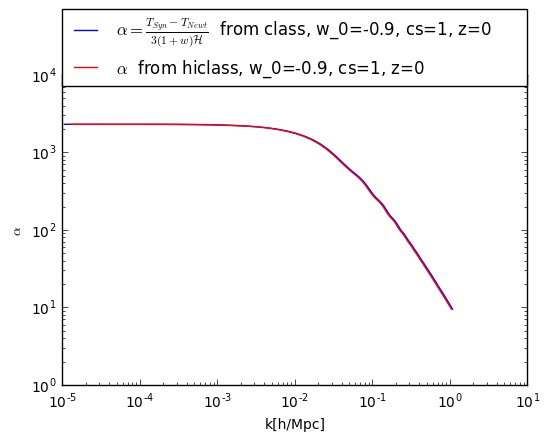
\includegraphics[width=0.60\textwidth]{alpha_class} 
\caption{The  $\alpha$ is in hi-class and class is compared. As it is clear they agree well. }
%\label{f1}
\end{center}
\end{figure}
%\begin{figure}[htbp!]
%\begin{center}
%\captionsetup{,margin=1cm}
%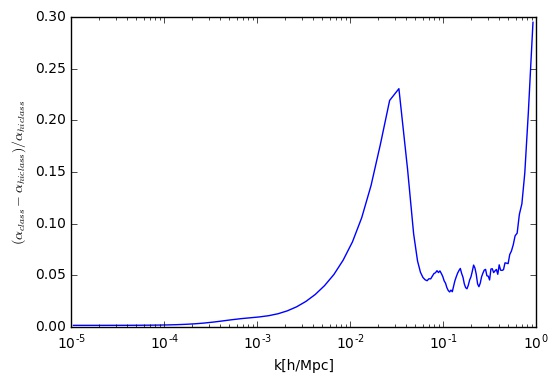
\includegraphics[width=0.60\textwidth]{alphaerror} 
%\caption{The  relative error of $\alpha$ in class and hi-class is shown. It is clear that  the relative error is very large in high wavenumbers.}
%%\label{plt2}
%\end{center}
%\end{figure}
So we have,
\be
\delta_{Newt}= \frac{1+w}{c_s^2} \Big ( -c_s^2 \mathcal{H} (\pi_{synch} + \alpha)- \mathcal{H} \alpha+\pi'_{synch}  \Big )
\ee
\be
\delta_{Synch}= \delta_{newt} + 3 \mathcal{H} (1+w) \alpha
\ee
\subsection{comparing the $\Psi$ function in Newtonian and synchronous gauge in class and hi-class}
Here we compare the metric fluctuation $\Psi$  in Newtonian gauge with one we obtain from Synchronous gauge parameters in class and hi-class codes to make sure we are dealing with the same functions. The $\Psi$ in Synchronous gauge reads as following,
\be
\Psi=\frac{1}{k^2} \Big [ {h^{''}}+ 6 {\eta^{''}} + \frac{a'}{a}  (h'+6 \eta ') \Big]= \alpha' + \mathcal{H}\alpha
\ee
In the figure \ref{psicomp} we compare the $\Psi$ in Newtonian gauge from what we get in terms of Synchronous gauge quantities.
\begin{figure}[H]
\begin{center}
\captionsetup{,margin=1cm}
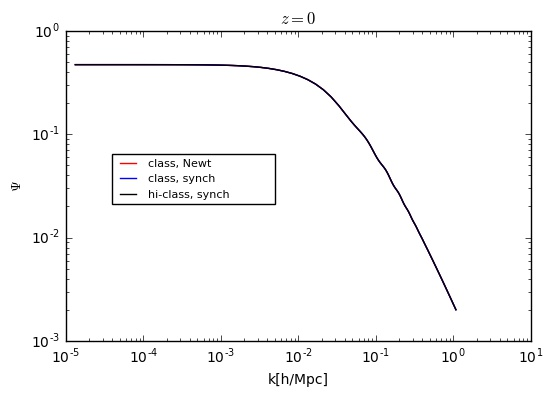
\includegraphics[width=0.60\textwidth]{psi_comp.jpg} 
\caption{$\Psi$ in Newtonian gauge and synchronous gauge in class and hi-class are compared. They all agree. }
\label{psicomp}
\end{center}
\end{figure}

\subsection{Comparing the  ${\pi}$ transfer function directly from hi-class and what we get from class indirectly}
From the equation for $\theta$, equation \ref{imp_2} we can obtain $\pi$ in Fourier space,
\be
\pi_{newt}=\frac{\theta_k\text{(newt)}}{k^2}  \; \; \; \text{(class)}
\ee
while in the hi-class we can easily obtain $\pi_{newt}$ by gauge transformation as following,
\be
\pi_{newt}= \pi_{synch}+ \alpha
\ee
An important key is that k in hi-class internally is in $1/Mpc$ unit while is class output is $h/Mpc$.\\
We assume two different models, one with $w_0=-0.9, c_s^2=1$ and the other with $w_0=-0.9, c_s^2=10^{-6}$ and we compare the results in both gauges. %The normalization factor in EFTcamb is assumed $\mathcal{H}$ and in class and hi-class the transfer function is assumed to be normalized to curvature function $\mathcal{R}$. So in the figure we have multiplied the EFTcamb result to $\mathcal{H}$ , hi-class and class result to $\delta_{\mathcal{R}}(k)= \frac{\sqrt{2 \pi^2 A_s(\frac{k}{k_p})^{n_s-1}}}{k^{3/2}}$.
\begin{figure}[H]
\begin{center}
\captionsetup{,margin=1cm}
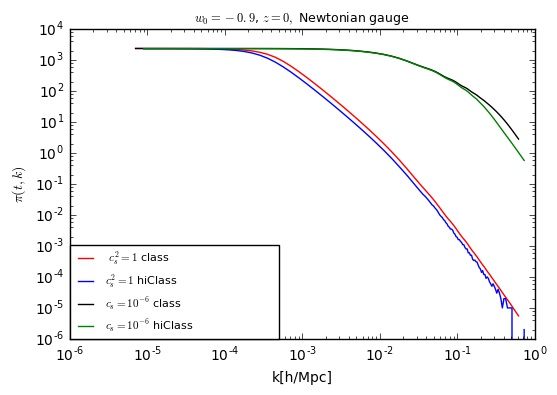
\includegraphics[width=0.60\textwidth]{pi_comp} 
\caption{$\pi$ comparison in Newtonian gauge for $w_0=-0.9, c_s^2=1$. Note that here we have use wrong gauge transformation for $\pi$ with different sign}
%\label{plt2}
\end{center}
\end{figure}


\subsection{Test 2: Density transfer in the limit of $c_s^2 \rightarrow 0 , w \rightarrow -1$ which should be the same as matter density transfer function}
In the limit of zero sound speed and $w_0 \rightarrow -1$ we expect that the k-essence field behave like dark matter. In the fluid description in the class it can be seen easily. In the below figure the density contrast transfer function for k-essence fluid and dark matter fluid is plotted. \\
We expect the same behaviour for the obtained k-essence field from hi-class or EFTcamb. So a good criterion is checking the behaviour in the mentioned limit.
\begin{figure}[H]
\begin{center}
\captionsetup{,margin=1cm}
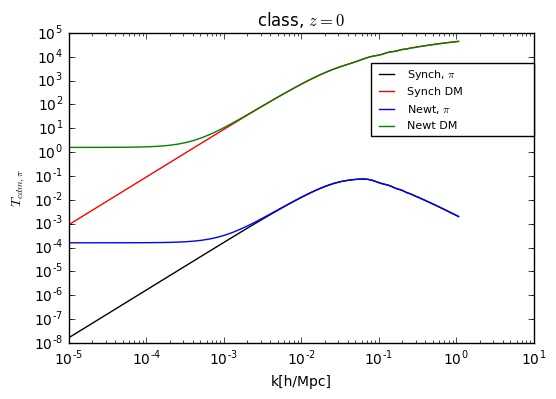
\includegraphics[width=0.60\textwidth]{cs0w1_fld.jpg} 
\caption{The behaviour of fluid and dark matter transfer function in the zero sound speed and $w_0 =-1$ limit is shown.  }
%\label{psicomp}
\end{center}
\end{figure}
Now we want to compare the result of density contrast transfer function of k-essence field in EFTcamb and hi-class with density contrast transfer of  fluid in the class. \\
I do not need to do this part, since I get good results in previous section.
%The density constrast $\delta$ in the EFTcamb and hi-class is calculated,
%\be
%\delta=\frac{1+w_0}{c_s^2} (\pi'- \Psi) =10^4 (\pi'- \Psi)
%\ee
%As we have checked $\Psi$ is the same in Class and hi-class so we can use $\Psi$ to obtain the $\delta$ of EFTcamb as well.
\subsection{Comparing the  ${\pi'}$ transfer function directly from hi-class and what we get from class indirectly}
Here we use $\delta$ transfer function from the Class output to construct $\pi'$ in Newtonian gauge. We get help of equation \ref{deltaeq} to reconstruct $\pi'$ as following,
\be
\pi'_{newt}= \frac{c_s^2}{1+w} \delta_{newt} + c_s^2 \mathcal{H} \frac{\theta_{newt}}{k^2} +\Psi
\ee
The we compare the result with what we get from the hi-class after gauge transformation as following,
\be
\pi'_{Newt} =\pi'_{Sync}+\alpha'
\ee
\subsection{Comparison of field transfer functions in the hi-class and the EFTcamb}
Now we want to use EFTcamb results for the k-essence which is straightforward to get the output , \\
%{\color{red} If we use pureEFT flag in EFTcamb, what are the related parameters for k-essence case?  since the translation between the standard language with EFTcamb is not trivial according to table 1 of   \url{https://arxiv.org/pdf/1411.3712.pdf} }
%In the beginning we use minimally coupled quintessence flag in the EFTcamb to check the consistency, then we should try the pureEFT flag. We choose the quintessence flag according to \url{http://www.eftcamb.org/images/EFTCAMB_structure.pdf} in the second part.
The result of comparison is shown in the following plot which shows that the two plot do not agree.
\begin{figure}[H]
\begin{center}
\captionsetup{,margin=1cm}
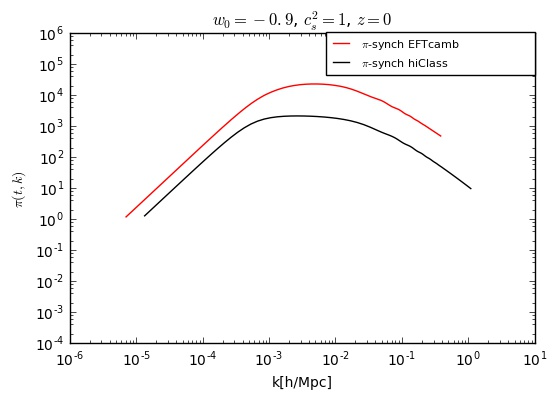
\includegraphics[width=0.60\textwidth]{eft_hiclass.jpg} 
\caption{EFTcamb and hi-class comparison.Here we compare the $\pi$ in Synchronous gauge. $1/\mathcal{H}$ is used as a  normalization factor for EFTcamb and k in hiclass is divided by h to be measures in $h/Mpc$.}
%\label{psicomp}
\end{center}
\end{figure}

\section{Gevolution}
\subsection{Initial condition}
All the transfer functions in the class and hi-class are normalized to one curvature perturbation. Curvature perturbation is obtained from powerspectrum as following,
\be
{\langle \mathcal{R} (k)  \mathcal{R} (k')\rangle} = (2 \pi )^3 \delta_D(k-k') P_{\mathcal{R}} (k)= (2 \pi )^3 \delta_D(k-k')  \frac{2 \pi^2}{k^3} \mathcal{P}_{\mathcal{R}}(k) =  (2 \pi )^3 \delta_D(k-k')   \frac{2 \pi^2}{k^3} A_s (\frac{k}{k_p})^{n_s-1}
\ee
So we can write
\be
\delta_{\mathcal{R}}(k)= \frac{\sqrt{2 \pi^2 A_s(\frac{k}{k_p})^{n_s-1}}}{k^{3/2}}
\ee
So $\delta_{\mathcal{R}}$, curvature perturbation transfer function, is the normalization factor which we should consider. Precisely we should multiply the field value from the class to $\delta_{\mathcal{R}}(k)$ to go in Gevolution units.\\
On the other hand, in the Gevolution after realization of the field the power spectrum is calculated as following,
\be
\langle \pi(k,t)  \pi(k,t) \rangle =(2 \pi )^3  P_{\pi} ^{Gev}=(2 \pi )^3   \delta_{\mathcal{R}}(k) ^2 P_{\pi}^{\text{hiclass}} = \frac{2 \pi^2}{k^3} A_s (\frac{k}{k_p})^{n_s-1} P_{\pi}^{\text{hiclass}}
\ee
In the Gevolution the wavenumber is measured in $\frac{h}{Mpc}$ but for the purpose of working with normal numbers it is multiplied to Boxsize so;
\be
k  \, \left[\frac{h}{Mpc} \right] = {k \times \text{Boxsize }}\, \left [\frac{{h}}{ \text{Boxsize }Mpc} \right]
\ee
As the powerspectrum in Gevolution in in $Mpc^3$ so $P(k[\frac{h}{Mpc}]) [\frac{Mpc^3}{h^3}]=P(k \, h [\frac{1}{Mpc}]) \left [{Mpc^3} \right ] $
%Plus in the gevolution $\frac{\text{Boxsize}}{Mpc}= \text{Number of grid points}$ 
The dimensionless powerspectrum is calculated as following: {(\color{red}{arXiv:0712.3028v2}}) \\
1- For the boxsize $L$, the field in Fourier space is discrete (no matter it is continuos or discrete in real space) and the k-modes are $\vec{k}= (\frac{2 \pi}{L}) (i,j,k)$. \\
2- The discrete Fourier transform is obtained by placing $\delta (x)$ on a lattice of  $N^3$ grid points with spacing $\frac{L}{N}$ 
\be
\delta_k^{DFT}= \frac{1}{N^3} \sum_r e^{-i\vec{k}.{r}} \delta(\vec{r})
\ee
3- Note that,
\be
\delta_k \approx ( \frac{\Delta x}{2 \pi} )^3 N^3 \delta_k^{DFT} \approx \dfrac{1}{\Delta k} \delta_k^{DFT} 
\ee
3- The powerspectrum is;
\be
P(k) \approx \frac{\langle | \delta^{DFT} |^2 \rangle}{(\Delta k)^3}
\ee
 4- The relation between dimensionless powerspectrum with the power with dimension is as following,
 \be
 \mathcal{P} (k)= \frac{k^3}{2 \pi ^2} P (k)
 \ee
 But factor $\frac{1}{N^6}$ should not be considered when we want to compare initial field transfer function with output powerspectrum! It is something internal in the Gevolution for calculating power from the realization. \\
 
-{\color{red}{Question:}} Why we do not get the same field realization (or order of magnitude) after going forward and backward in Fourier space? \\
- Is the below code right for realizing the field in Fourier and real space?
\begin{lstlisting}
generateRealization(*scalarFT_pi, 0., tk_d_kess, (unsigned int) ic.seed,
 ic.flags & ICFLAG_KSPHERE); 
plan_pi_k ->execute(FFT_BACKWARD);
pi_k->updateHalo();	// pi_k now is realized in real space
plan_pi_k->execute(FFT_FORWARD);}
\end{lstlisting}
If we turn off the following part we get completely different solution for the field in real space! As we expect the same order of magnitude of the $\pi (t,\vec{x})$ as other perturbations field $\phi$ so it seems we should turn off the below command! 
\begin{lstlisting}
plan_pi_k->execute(FFT_FORWARD); 
\end{lstlisting}
\subsection{Gevolution initial field factors from initial condition to output power }
When we give the field transfer function as an initial condition in Gevolution, since in class it is normalized to $\mathcal{R}$ curvature perturbation, first we need to multiply to $\sqrt{P_{\mathcal{R}}}$. On the other hand we need to notice to the units of $k$ in input initial condition and what Gevolution work with internally. \\
What happens in the $icbasic.hpp$,
\be
\pi_{gev} = -\sqrt{2} \times \pi_{numb} \; \; \;\frac{ \pi_{class} \sqrt{\mathcal{P}_{\mathcal{R}}(k/ \text{Boxsize})  }} {k[h/Mpc]^{3/2}}
\ee
Note that the factor $\sqrt{2}$ in the above definition is missed in Gevolution! Actually it is recovered in the output power for other variables. So we keep the convention and use the below formula,
\be
\pi_{gev} = - \pi_{numb} \; \; \;\frac{ \pi_{class} \sqrt{\mathcal{P}_{\mathcal{R}}(k/ \text{Boxsize})  }} {k[h/Mpc]^{3/2}}
\ee
{\color{red} What is the negative sign here?}
\\
Where $\mathcal{P}_{\mathcal{R}}=A_s (\frac{k}{k_p})^{n_s-1}$ in the code internally, $k_p$ is in the unit of $1/Mpc$ and $\mathcal{P}_{\mathcal{R}}$ is dimensionless.
and $\pi_{numb}$ $\pi$ number. \\
In order to know why we divide by $k[h/Mpc]^{3/2}$ we need to look at other part of the code to get what happens...\\
Boxsize in gevolution is $Mpc/h$. So its better to give k in class in $h/Mpc$.
\be
k_{gev}= k_{class} [h/Mpc] \text{Boxsize}[Mpc/h]
\ee
So k when it is read out is dimensionless, equivalently it is in comoving box. \\
Moreover the quantities in class and hiclass are normalized to dimensionful curvature perturbation so the coefficient in Gevolution is,
\be
\delta_{\mathcal{R}}(k)= \frac{\sqrt{2 \pi^2 A_s(\frac{k}{k_p})^{n_s-1}}}{k^{3/2}}
\ee
More over it is very important to note that since $\pi$ in class has dimension $Mpc$ is not enough to divide by Boxsize in Gevolution since it is actually in the unit of $1/H$ where in Gevolution it is divided by c light velocity. To make it consistent we do $\pi \mathcal{H}_{class}/\mathcal{H}_{Gev}$ since $\pi \mathcal{H}_{class}$ is dimensionless in class and we make it in time dimension in Gevolution by dividing to $\mathcal{H}_{Gev}$
\\
\subsection{writePowerSpectrum}
Now we want to extract writePowerSpectrum function where the coefficients are very important. \\
First of all  we have k which is in unit of boxsize must divided by boxsize to give $h/Mpc$ unit. Unit conversion for P (power) depends on the quantity but $\frac{1}{N_{points}^6 \times 2 \pi^2}$ is common. $N_{points}^6$ comes from FFT definition, $2 \pi^2$. \\
{\color{red} Here everything is so confusing! I do not know why $\sqrt{2}$ in the definition of $\delta_{\mathcal{R}}$ is missed, I also do not know why at the end it is not multiplied to $\frac{k^3}{2 \pi ^2}$, also negative sign in the definitions!!! it seems that  something is done internally that I cannot track well!!!}. \\
What I'm doing is following the same notation and then check what is going on and do some consistency checks!!


 \subsection{Stress tensor}
{ \color{red}{ Todo: How to add stress tensor?}} \\
Should  
{\begin{lstlisting}
projection_init(&source); 
\end{lstlisting}}
contains the scalar field in it?\\
- what is source and where it is calculated? \\
- Is it $T_\mu^{\nu}$ or $T_{\mu \nu} $in Gevolution?\\
-what is the meaning of below lines before the functions definitions.
{\begin{lstlisting}
-template<typename part, typename part_info, typename part_dataType>
template <class FieldType>
\end{lstlisting}}
 \subsection{Field equation and transfer}
 { \color{red}{ Todo: use the correct field equation and check the transfer function in time?}}
 \subsection{Some tests on Gevolution:}
 We want to test if the initial powerspectrum is the same as realized field powerspectrum in gevolution. \\
 In the figure \ref{comparehi-gev} the powerspectrum of the field from Gevolution's output is compared with the one which is made by hand. We make the dimensionless powerspectrum by hand from the initial transfer function as following,
 \be
 \mathcal{P}_{\pi}^{Gevolution} (k) = \frac{k ^3}{2 \pi ^2} \; \delta_{\mathcal{R}}^2 \,  \delta_{\pi}
^{\text{hiclass}} \times  \delta_{\pi}^{\text{hiclass}} =  \frac{k ^3}{2 \pi ^2} \;    \frac{2 \pi^2 A_s(\frac{k}{k_p})^{n_s-1}}{k^{3}}  \;  \delta_{\pi}
^{\text{hiclass}} \times  \delta_{\pi}^{\text{hiclass}} =    { A_s(\frac{k}{k_p})^{n_s-1}} \;  \delta_{\pi}
^{\text{hiclass}} \times  \delta_{\pi}^{\text{hiclass}} 
 \ee
 \begin{figure}[htbp!]
\begin{center}
\captionsetup{,margin=1cm}
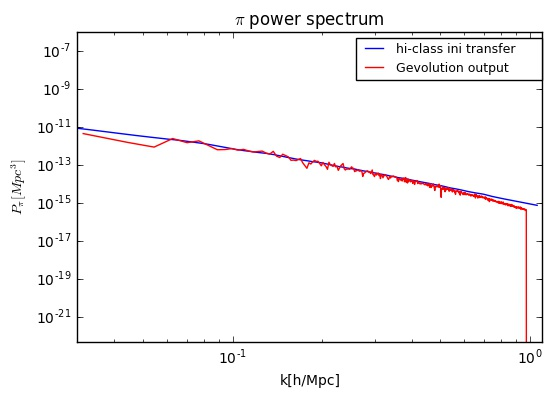
\includegraphics[width=0.60\textwidth]{Gev-hiclass} 
\caption{The powerspectrum which is calculated by hand is compared with output power of Gevolution. Simulation setting is: Boxsize=200 $Mpc/h$,  N$\_$grid=64 .  There is a deviation between two plots in high wavenumbers { \color{Red}{why?}}. While the Nyqvist frequency approximately is $\frac{2 \pi }{\Delta x} \approx  \frac{2 \pi \times \text{num}-{\text{grids}} }{\text{Boxsize}} =2.01 \, \frac{h}{Mpc}$}
\label{comparehi-gev}
\end{center}
\end{figure}
 Note that to get $H0$ in class unit, we have $H0=\frac{100h \times 10^3}{3 \times 10^8} [1/Mpc]$ where the first $10^3$ is because of $km/s$ and is divided by c. \\
 It is also important to note that, to obtain $\pi$ from $\delta $ and $\theta$ in class, because we have $H \pi_{phys}$ combination and since it is dimensionless we have $\mathcal{H} \pi_{conf} = H \pi_{phys}$. \\
 Also $\theta=-\nabla^2 \pi_{conf}=-\nabla^2 \pi_{phy}/a^2$ and negative sign is the convention. \\
 In Gevolution $H_{0}=\sqrt{8 \pi G/3}$ since $\rho_{crit}^0=1$ and also note that we have $4 \pi G= \frac{3 \text{Boxsize}^2}{2 c^2}$, in order for working with normal numbers internally, and $c[100km/s]$ in the code.
 
 \section{K-essence field equation from EFT action}
Here we use the second order EFT action and vary it with respect to the field and we obtain the equations with leading order post Newtonian corrections, \\
The action is as following,
\be
S=\sqrt{-g} \left [ \frac{M_*^2}{2} f(t) R -\Lambda (t) -c(t) g^{00} +\frac{M_2^4(t)}{2} \left (g^{00} + \frac{1}{\bar{N}^2} \right )    -  \frac{m_3^3(t)}{2} \delta K  \left (g^{00} + \frac{1}{\bar{N}^2} \right )    \right ]
\ee
We recover the full covariance with second order Stuckelberg trick,
\be
f(t) \longrightarrow f(t) +  \dot{f} (t) \pi+ \frac{1}{2} \ddot{f }(t) \pi^2  + \frac{1}{6} \dddot{f }(t) \pi^3
\ee
\be
\Lambda(t) \longrightarrow \Lambda(t) +  \dot{\Lambda} (t) \pi+ \frac{1}{2} \ddot{\Lambda}(t) \pi^2 + \frac{1}{6} \dddot{\Lambda }(t) \pi^3
\ee
\be
M_2^4(t) \longrightarrow M_2^4(t) +  \dot{ M_2^4} (t) \pi+ \frac{1}{2}    \ddot{ M_2^4 }(t)  \pi^2 + \frac{1}{6} \dddot{M_2^4 }(t) \pi^3
\ee
\be
m_3^3(t) \longrightarrow m_3^3(t) +  \dot{m_3^3} (t) \pi+ \frac{1}{2} \ddot{m_3^3}(t) \pi^2 + \frac{1}{6} \dddot{m_3^3 }(t) \pi^3
\ee
\be
g^{00} \longrightarrow g^{00} + 2 g^{0 \mu} \partial_{\mu} \pi + g^{\rho \nu} \partial_{\rho} \partial_{\nu} \pi
\ee
\begin{align}
\delta K  \longrightarrow &   \delta K -3 \left ( \dot{H} \pi +\frac{1}{2} \ddot{H} \pi^2 \right ) - (1-\dot{\pi}) N h^{ij} \partial_i \partial_j \pi +\frac{1}{2} \partial_i h^{ij} \partial_j \pi  \nonumber \\ &+\frac{H}{2 a^2} \delta ^{ij}\partial_i \pi \partial_j \pi + \frac{2}{a^2} \delta ^{ij} \partial_i  \pi  \partial_j    \dot{\pi} -\frac{2}{a^2} \delta ^{ij} \partial_i N \partial_j \pi
\end{align}
\begin{align}
\frac{1}{\sqrt{-g}} \frac{\delta S}{\delta \pi}|_{\text{First order} }&=  B_{\Psi} \Psi+  B_{\dot{\Psi}} \dot{\Psi} +
B_{\Phi} \Phi + B_{\dot{\Phi}} \dot{\Phi}  + B_{\ddot{\Phi}} \ddot{\Phi}+B_{\pi} \pi +   B_{\dot{\pi}} \dot{\pi} + B_{\ddot{\pi}} \ddot{\pi}  
\nonumber  \\& 
+ \frac{k^2}{a^2} \left( B^{(2)}_{\Psi}\Psi +  B^{(2)}_{\Phi}\Phi+ B^{(2)}_{\dot{\Phi}} \dot{\Phi} + B^{(2)}_{\pi}\pi \right) + \frac{k^4}{a^4} \left(B^{(4)}_{\Phi}\Phi +B^{(4)}_{\pi}\pi  \right)
\end{align}
where,
\be
B_{\Psi}=12 c H+2 \dot{c} +3 m_3^3 (3H^2+2\dot{H}) -6 M_*^2\dot{f} (\dot{H} + 2H^2) + 3H \left[ 4M_2^4 +\dot{(m_3^3)}\right]+4 \dot{(M_2^4)}
\ee
The last equation is different with Essential building paper, because of a typo in the paper.
\be
B_{\dot{\Psi}}=2c + 4 M_2^4 +3 H (m_3^3 -M_*^2 \dot{f})
\ee
\be
B_{\Phi}=0
\ee
\be
B_{\dot{\Phi}}=3 \left[ 2c +3 H m_3^3-4 H M_*^2 \dot{f} +\dot{m_3^3}\right]
\ee
\be
B_{\ddot{\Phi}}=3( m_3^3 -M_*^2 \dot{f})
\ee
\be
B_{{\pi}}=- \Big[ -3\dot{m_3^3} \dot{H} + 6 \dot{H} c + 3 M_*^2 (\ddot{H} +4 H \dot{H})\dot{f} - 9 H \dot{H} m_3^3- 3 m_3^3 \ddot{H}  \Big]
\ee
\be
B_{\dot{\pi}}=- 2\Big[ 3 H (c+ 2 M_2^4) +\dot{c} + 2\dot{M_2^4} \Big]
\ee
\be
B_{\ddot{\pi}}=- 2\Big[  c+ 2 M_2^4 \Big]
\ee
\be
B^{(2)}_{{\Psi}}=- \Big[  m_3^3 + H (- 6 H \bar{m}_5+4 \tilde{m}_4^2) - M_*^2 \dot{f}\Big]
\ee
\be
B^{(2)}_{{\Phi}}=- 2\Big[ 2 H \tilde{m}_4^2 + M_*^2 \dot{f}-3 \bar{m}_5 \dot{H} + 2 \dot{(\tilde{m}}_4^2) \Big]
\ee
\be
B^{(2)}_{\dot{\Phi}}=
  6H \bar{m}_5 - 4 \tilde{m}_4^2
\ee
\be
B^{(2)}_{{\pi}}=
- \Big[ 2c + 4 \tilde{m}_4^2 \dot{H} + \dot{m_3^3}+ 4 H^2 \tilde{m}_4^2+ H m_3^3 -12 \bar{m}_5 H \dot{H} + 4 H \dot{(\tilde{m}}_4^2)\Big]
\ee
\be
B^{(4)}_{{\Phi}}=-2 \bar{m} _5 + 16 H \bar{\lambda}
\ee
\be
B^{(4)}_{{\pi}}=
-2(\bar{m}_4^2 +2 H \bar{m}_5)+ 16 H^2 \bar{\lambda}
\ee
The relevant second order terms in Fourier space are,
\begin{align}
\frac{1}{\sqrt{-g}} \frac{\delta S}{\delta \pi}|_{\text{post newtonian} }&=  \int \int d^3k d^3 k' e^{i(\vec{k}+\vec{k}') . \vec{x}}  \Bigg [   -\frac{k^2}{a^2} C^{(2)}_{\Psi \Psi} \Psi \Psi  -\frac{k^2}{a^2} C^{(2)}_{\Psi \Phi} \Psi \Phi   -\frac{k^2}{a^2} C^{(2)}_{\Psi \pi} \Psi \pi 
  -\frac{k^2}{a^2} C^{(2)}_{\Phi \Psi} \Phi \Psi  -\frac{k^2}{a^2} C^{(2)}_{\Phi \Phi} \Phi \Phi   -\frac{k^2}{a^2} C^{(2)}_{\Phi \pi} \Phi \pi 
\nonumber  \\& 
   -\frac{k^2}{a^2} C^{(2)}_{\pi \Psi} \pi \Psi  -\frac{k^2}{a^2} C^{(2)}_{\pi \Phi} \pi \Phi   -\frac{k^2}{a^2} C^{(2)}_{\pi \pi} \pi \pi 
  -\frac{k^2}{a^2} C^{(2)}_{\dot{\Psi} \Psi} \dot{\Psi} \Psi  -\frac{k^2}{a^2} C^{(2)}_{\dot{\Psi} \Phi} \dot{\Psi} \Phi   -\frac{k^2}{a^2} C^{(2)}_{\dot{\Psi} \pi} \dot{\Psi} \pi 
\nonumber   \\&
 -\frac{k^2}{a^2} C^{(2)}_{\dot{\Phi} \Psi} \dot{\Phi} \Psi  -\frac{k^2}{a^2} C^{(2)}_{\dot{\Phi} \Phi} \dot{\Phi} \Phi   -\frac{k^2}{a^2} C^{(2)}_{\dot{\Phi} \pi} \dot{\Phi} \pi 
  +C_{ \dot{\pi}\dot{\pi}}  \dot{\pi}\dot{\pi}  -\frac{k^2}{a^2} C^{(2)}_{\dot{\pi} \Psi} \dot{\pi} \Psi  -\frac{k^2}{a^2} C^{(2)}_{\dot{\pi} \Phi} \dot{\pi} \Phi   -\frac{k^2}{a^2} C^{(2)}_{\dot{\pi} \pi} \dot{\pi} \pi \text{ .}
    \nonumber \\&
  -\frac{\vec{k}.\vec{k}'}{a^2}  C^{1,1}_{\Psi \Phi} \Psi \Phi  -\frac{\vec{k}.\vec{k}'}{a^2}  C^{1,1}_{\Psi \pi} \Psi \pi  -\frac{\vec{k}.\vec{k}'}{a^2}  C^{1,1}_{\Phi \pi} \Phi \pi  -\frac{\vec{k}.\vec{k}'}{a^2}  C^{1,1}_{\pi \pi} \pi \pi   -\frac{\vec{k}.\vec{k}'}{a^2}  C^{1,1}_{\Psi \Psi} \Psi \Psi -\frac{\vec{k}.\vec{k}'}{a^2}  C^{1,1}_{\Phi \Phi} \Phi \Phi    
  \nonumber \\ &
 + C_{\ddot{\Psi}} (\Psi,\Phi,\pi) \ddot{\Psi} + C_{\ddot{\Phi}} (\Psi,\Phi,\pi) \ddot{\Phi}+ C_{\ddot{\pi}} (\Psi,\Phi,\pi) \ddot{\pi} \Bigg ] 
  \text{ .}
\end{align}
Where;
\be
C^{(2)}_{\Psi \Psi}=  - m_3^3 \text{ .}
\ee
\be
C^{(2)}_{\Psi \Phi}= 0 \text{ .}
\ee
\be
C^{(2)}_{\Psi \pi}=  -4 H m_3^3 - 4 M_2^4  \text{ .}
\ee
\be
C^{(2)}_{\Phi \Psi}= 2 (m_3^3 -M_*^2 \dot{f})  \text{ .}
\ee
\be
C^{(2)}_{\Phi \Phi}= 4 M_*^2 \dot{f} \text{ .}
\ee
\be
C^{(2)}_{\Phi \pi}= 2 \left ( m_3^3 H + 2 c +\dot{m_3^3}  \right )   \text{ .}
\ee
\be
C^{(2)}_{\pi \Psi}= \dot{m_3^3} - M_*^2 \ddot{f} \text{ .}
\ee
\be
C^{(2)}_{\pi \Phi}= 2 M_*^2 \ddot{f} \text{ .}
\ee
\be
C^{(2)}_{\pi \pi}=  -3m_3^3 \dot{H} +  H \dot{m_3^3} + 2 \dot{c} +  \ddot{m_3^3}   \text{ .}
\ee
\be
C^{(2)}_{\dot{\Psi} \Psi}= 0\text{ .}
\ee
\be
C^{(2)}_{\dot{\Psi} \Phi}=0 \text{ .}
\ee
\be
C^{(2)}_{\dot{\Psi} \pi}= -m_3^3 \text{ .}
\ee
\be
C^{(2)}_{\dot{\Phi} \Psi}=0 \text{ .}
\ee
\be
C^{(2)}_{\dot{\Phi} \Phi}=0 \text{ .}
\ee
\be
C^{(2)}_{\dot{\Phi} \pi}= -4 m_3^3 \text{ .}
\ee
\be
C^{(2)}_{\dot{\pi} \Psi}= m_3^3   \text{ .}
\ee
\be
C^{(2)}_{\dot{\pi} \Phi}= 0 \text{ .}
\ee
\be
C^{(2)}_{\dot{\pi} \pi}= 4 M_2^4 \text{ .}
\ee
\be
C^{1,1}_{\Psi \Phi}= - (m_3^3 -M_*^2 \dot{f}) \text{ .}
\ee
\be
C^{1,1}_{\Psi \pi}=  2 (-m_3^3 H + c- 2 M_2^4 +\dot{m_3^3 })    \text{ .}
\ee
\be
C^{1,1}_{\Phi \pi}= - \left (  m_3^3 H + 2c + \dot{m_3^3}  \right )      \text{ .}
\ee
\be
C^{1,1}_{\Phi \Phi}=	- M_*^2 \dot{f}	\text{ .}
\ee
\be
C^{1,1}_{\pi \pi}= \frac{1}{2} \left (  3 m_3^3 H^2 + 2 (\dot{c} +2  \dot{M_2^4})+ 4 M_2^4 H - H \dot{m_3^3 }  -4 {m_3^3}  (H^2 +\dot{H}) \right )	\text{ .}
\ee
\be
C^{1,1}_{\Psi \Psi}= - M_*^2 \dot{f}	\text{ .}
\ee
\be
C_{\ddot{\Psi}} (\Psi,\Phi,\pi)=0	\text{ .}
\ee
\be
C_{\ddot{\Phi}} (\Psi,\Phi,\pi)= 0 \text{ .}
\ee
\be
C_{\ddot{\pi}} (\Psi,\Phi,\pi)= 	- m_3^3 \frac{k^2}{a^2} \tilde{\pi} \text{ .}
\ee
For the k-essence case we have (note below equation 85 in \url{https://arxiv.org/pdf/1411.3712.pdf})
\begin{align}
& \alpha_B= \alpha_H=\alpha_M=\alpha_T=0 \nonumber \\ &
\alpha_K=\frac{2\bar{X} P _X + 4 \bar{X}^2 P_{XX}}{M^2 H^2 }  \nonumber \\ &
c_s^2=\frac{-2 \dot{H}}{\alpha_K H^2 } - \frac{\rho + P}{\alpha_K M^2 H^2}
\end{align}
After translation between two different language according to table 1 of  \url{https://arxiv.org/pdf/1411.3712.pdf} and equation 24-25 of \url{https://arxiv.org/pdf/1210.0201.pdf} we get,
\begin{align}
 & m_4^2=\tilde{m}_4^2=\bar{\lambda}=0 \nonumber  \\ &
 f=1 \longrightarrow M^2=3M_{pl}^2,  \;  \;  m_3^3=0 , \;  \; \alpha_k=\frac{2c +4 M_2^4}{M^2 H^2}=  \frac{\Omega (1+w)}{c_s^2} \\ \nonumber &
 \Lambda= -\frac{\bar{\rho} (1-w)}{2}, \; \; c=\frac{\bar{\rho} (1+w)}{2}, \; \; 4 M_2^4=\bar{\rho} (1+w) (\frac{1}{c_s^2}-1)
\end{align}
\subsection{Friedmann equations}
In this language the Friedman equations are,
\be
3{H}^2 M_{pl}^2= \rho_m + \rho_{scf}
\ee
Note that in Gevolution we have,
\be
\mathcal{H}^2=\frac{8 \pi G}{3} (\Omega_m a^{-3} +\Omega_{rad} a^{-4} +\Omega_{kess} a^{-3(1+w)} +\Omega_L a^{0} ) \times a^2
\ee
Where the critical density in here assumed 1, ie. $H_0^2=\mathcal{H}_0^2=\frac{8 \pi G}{3}$
and 
\begin{align}
&\frac{\ddot{a}}{a} = - \frac{1}{6M^2_{pl}} \left (\rho_{tot} +3 P_{tot}\right ) \\ \nonumber &
3 H^2 + 2\dot{H} = \frac{-1}{M^2_{pl}} \left( P_{m} + P_{scf} (X, \varphi) \right)
\end{align}
Equivalently it can be written,
\be
\dot{H}= \frac{-(2 \bar{X} P_{,X} + \rho_m+ P_m)}{6 M^2_{pl}}
\ee
where
\be
\bar{X}=\frac{1}{2} \; \; P_{,X} = \bar{\rho} (1+w)
\ee
which is the same as equation 3.5 of \url{https://arxiv.org/pdf/1404.3713.pdf} 
The non-zero terms are:\\
{\color{red} Note that it is assumed that "w" is constant, $\bar{\rho}$ is density of k-essence field and continuity equation for k-essence field is $\dot{\bar{\rho}} +3 H \bar{\rho} (1+w)=0 $}
\be
B_{\Psi}=12 c H+2 \dot{c}  + 3H ( 4M_2^4)+4 \dot{(M_2^4)} =  \frac{\dot{\bar{\rho}} (1+w)}{c_s^2} + 3 {H} \bar{\rho} (1+w) \Big( \frac{1}{c_s^2}+1 \Big)=3 {H} \bar{\rho} (1+w) \Big( 1- \frac{w}{c_s^2} \Big )
\ee
\be
B_{\dot{\Psi}}=2c + 4 M_2^4 =  \frac{\bar{\rho} (1+w)}{c_s^2}
\ee
\be
B_{\dot{\Phi}}=6 c = 3 \bar{\rho} (1+w)
\ee
\be
B_{{\pi}}=- 6 \dot{H} c= - 3 \dot{H} \bar{\rho} (1+w)
\ee
\be
B_{\dot{\pi}}=- 2\Big[ 3 H (c+ 2 M_2^4) +\dot{c} + 2\dot{M_2^4} \Big] = \frac{3 H w (1+w) \bar{\rho} }{c_s^2}
\ee
\be
B_{\ddot{\pi}}=- 2\Big[  c+ 2 M_2^4 \Big]=- \frac{  \bar{\rho}(1+w) }{c_s^2}
\ee
\be
B^{(2)}_{{\pi}}=
- 2c  =-\bar{\rho}(1+w) 
\ee
\be
C^{(2)}_{\Psi \pi}=  -\bar{\rho} (1+w) (\frac{1}{c_s^2}-1)
  \text{ .}
\ee
\be
C^{(2)}_{\Phi \pi}= 4 c =  2 \bar{\rho} (1+w) \text{ .}
\ee
\be
C^{(2)}_{\pi \pi}=    2 \dot{c} =\dot{\bar{\rho}}(1+w) =-3 H  \bar{\rho} (1+w) ^2  \text{ .}
\ee
\be
C^{(2)}_{\dot{\pi} \pi}=\bar{\rho} (1+w) (\frac{1}{c_s^2}-1) \text{ .}
\ee
\be
C^{1,1}_{\Psi \pi}=  2  c- 4 M_2^4 = \bar{\rho} (1+w) (2-\frac{1}{c_s^2})   \text{ .}
\ee
\be
C^{1,1}_{\Phi \pi}=-2c = -   \bar{\rho} (1+w)   \text{ .}
\ee
\be
C^{1,1}_{\pi \pi}= \frac{1}{2} \left (  2 (\dot{c} +2  \dot{M_2^4})+ 4 M_2^4 H\right )= -\frac{\bar{\rho} H (1+w)} {2 c_s^2} \Big(2+3w+c_s^2  \Big) 	\text{ .}
\ee
The final equation is:
\begin{align} 
 &3 {H} \bar{\rho} (1+w) \Big( 1- \frac{w}{c_s^2} \Big )
 \Psi + \frac{ \bar{\rho} (1+w)}{c_s^2} \dot{\Psi} + 3 \bar{\rho} (1+w) \dot{\Phi} -3 \dot{H} \bar{\rho} (1+w) \pi + \frac{3 {H} \bar{\rho} (1+w) w}{c_s^2} \dot{\pi} -\frac{  \bar{\rho} (1+w)}{c_s^2} \ddot{\pi} + \bar{\rho} (1+w) \frac{\nabla^2 \pi}{a^2} \nonumber \\ 
 &
  -\bar{\rho} (1+w) (\frac{1}{c_s^2}-1)\pi \frac{\nabla^2 \Psi }{a^2} + 2\bar{\rho} (1+w) \pi \frac{\nabla^2 \Phi }{a^2}   - 3 H \bar{\rho} (1+w)^2 \pi \frac{\nabla^2 \pi }{a^2}    +  \bar{\rho} (1+w) (\frac{1}{c_s^2}-1)
   \pi \frac{\nabla^2 \dot{\pi }}{a^2}   
    \nonumber \\ &
   +\bar{\rho} (1+w) (2-\frac{1}{c_s^2}) \frac{\nabla  \Psi . \nabla \pi }{a^2}   
 - \bar{\rho} (1+w) \frac{\nabla  \Phi . \nabla \pi } {a^2}   -\frac{\bar{\rho} H (1+w)} {2 c_s^2} \Big(2+3w+c_s^2  \Big)\frac{\nabla  \pi . \nabla \pi } {a^2}     =0
  \end{align}
Simplifying the expression gives,
\begin{align} 
 & 3 {H}  \Big( 1- \frac{w}{c_s^2} \Big )
\Psi + \frac{ 1}{c_s^2} \dot{\Psi} + 3 \dot{\Phi} -3 \dot{H} \pi + \frac{3 {H} w}{c_s^2} \dot{\pi} -\frac{  1}{c_s^2} \ddot{\pi} + \frac{\nabla^2 \pi }{a^2}
     - (\frac{1}{c_s^2}-1)\pi \frac{\nabla^2 \Psi }{a^2} + 2 \pi \frac{\nabla^2 \Phi }{a^2}   - 3 H (1+w) \pi \frac{\nabla^2 \pi }{a^2}   
       \nonumber
   \\
    & +  (\frac{1}{c_s^2}-1)
   \pi \frac{\nabla^2 \dot{\pi }}{a^2}   
   + (2-\frac{1}{c_s^2}) \frac{\nabla  \Psi . \nabla \pi }{a^2}   
 - \frac{\nabla  \Phi . \nabla \pi } {a^2}   -\frac{H} {2 c_s^2} \Big(2+3w+c_s^2  \Big)\frac{\nabla  \pi . \nabla \pi } {a^2}     =0 \label{fineq}
%  -(\frac{1}{c_s^2}-1) \nabla^2 \Psi \pi+ 2 \nabla^2 \Phi \pi - 3 H (1+w) \pi \nabla^2 \pi  + (\frac{1}{c_s^2}-1) \pi \nabla^2 \dot{\pi}   \nonumber \\ &+ (2-\frac{1}{c_s^2})\nabla \Psi \nabla \pi - \nabla \Phi \nabla \pi -\frac{H} {2 c_s^2} \Big(2+3w+c_s^2  \Big) \nabla \pi \nabla \pi =0
  \end{align} 
  We have checked that the top equation agrees with equation 113 of \url{https://arxiv.org/pdf/1411.3712.pdf} up to first order. 
  \subsection{The equation in terms of conformal time}
  To express the last expression in terms of conformal time we only need to follow the following transformations, \\
  \be
  a d \tau= dt
  \ee
  The relation between Hubble and conformal Hubble is;
\be
\mathcal{H} (\tau)=\frac{1}{a(\tau) }\frac{d a(\tau)}{d \tau }= \frac{1}{a(t) } \frac{d a (t) }{d t} \frac{d t }{ d\tau}= a H(t)
\ee
and for the derivative,
\begin{align}
& \dot{H}= \frac{-\mathcal{H}^2+ \mathcal{H}'}{a^2} \nonumber \\ &
\mathcal{H}'=a^2 \Big[ H^2 + \dot{H}\Big ]
\end{align}
The time derivative of any function of time like $\pi(t)$ transforms as,
\be
\pi(x,t)=\pi(x,\tau)
\ee
\be
\dot{\pi}=\frac{\partial \pi}{\partial \tau}  \frac{\partial \tau}{\partial t} = \frac{1}{a(\tau)} \pi '
\ee
\be
\ddot{\pi}=\frac{\partial \tau}  {\partial t} \frac{\partial }{\partial \tau} (\frac{1}{a}\pi ' ) = \frac{1}{a} (-\frac{a ' \pi'}{a^2}+ \frac{\pi''}{a})= \frac{1}{a^2} \Big(- \mathcal{H} \pi' + \pi'' \Big)
\ee
So the equation \ref{fineq} becomes,
\begin{align} 
 & 3 \frac{\mathcal{H}
}{a} \Big( 1- \frac{w}{c_s^2} \Big )\Psi + \frac{ 1}{c_s^2} \frac{\Psi'}{a}+ 3 \frac{\Phi'}{a} -3  \frac{-\mathcal{H}^2 + \mathcal{H}'}{a^2} \pi + \frac{3 \mathcal{H} w}{ a c_s^2} \frac{\pi'}{a}  -\frac{  1}{ a^2 c_s^2} \Big(- \mathcal{H} \pi' + \pi'' \Big) + \frac{\nabla^2 \pi }{a^2}
     - (\frac{1}{c_s^2}-1)\pi \frac{\nabla^2 \Psi }{a^2} + 2 \pi \frac{\nabla^2 \Phi }{a^2}   - 3 H (1+w) \pi \frac{\nabla^2 \pi }{a^2}   
       \nonumber
   \\
    & +  (\frac{1}{c_s^2}-1)
   \pi \frac{\nabla^2\pi ' }{a^3}   
   + (2-\frac{1}{c_s^2}) \frac{\nabla  \Psi . \nabla \pi }{a^2}   
 - \frac{\nabla  \Phi . \nabla \pi } {a^2}   -\frac{\mathcal{H}} {2 a c_s^2} \Big(2+3w+c_s^2  \Big)\frac{\nabla  \pi . \nabla \pi } {a^2}     =0 \label{fineq}
%  -(\frac{1}{c_s^2}-1) \nabla^2 \Psi \pi+ 2 \nabla^2 \Phi \pi - 3 H (1+w) \pi \nabla^2 \pi  + (\frac{1}{c_s^2}-1) \pi \nabla^2 \dot{\pi}   \nonumber \\ &+ (2-\frac{1}{c_s^2})\nabla \Psi \nabla \pi - \nabla \Phi \nabla \pi -\frac{H} {2 c_s^2} \Big(2+3w+c_s^2  \Big) \nabla \pi \nabla \pi =0
  \end{align} 
  Multiplying to $-a^2 c_s^2$ gives:
  \begin{empheq}[box=\tcbhighmath]{equation}
 \begin{align} 
 &\pi'' - \mathcal{H} \Big (1+ 3w \Big)\pi' -3 {a c_s^2 \mathcal{H}}\Big( 1- \frac{w}{c_s^2} \Big )\Psi -a \, {\Psi'}- 3 c_s^2 a \,{\Phi'} 
  +3  c_s^2 \Big({-\mathcal{H}^2 + \mathcal{H}'} \Big) \pi 
 - c_s^2 {\nabla^2 \pi }
     + (1-c_s^2)\pi {\nabla^2 \Psi }
      - 2 c_s^2 \pi {\nabla^2 \Phi }
            \nonumber
   \\
    &
      + 3 c_s^2  H (1+w)\pi {\nabla^2 \pi }   
  -  (1-c_s^2)
   \pi \frac{\nabla^2\pi ' }{a}   
   - (2 c_s^2-1) {\nabla  \Psi . \nabla \pi }
 + c_s^2 {\nabla  \Phi . \nabla \pi }  
   +\frac{\mathcal{H}} {2 a } \Big(2+3w+c_s^2  \Big) \,{\nabla  \pi . \nabla \pi }     =0 
%  -(\frac{1}{c_s^2}-1) \nabla^2 \Psi \pi+ 2 \nabla^2 \Phi \pi - 3 H (1+w) \pi \nabla^2 \pi  + (\frac{1}{c_s^2}-1) \pi \nabla^2 \dot{\pi}   \nonumber \\ &+ (2-\frac{1}{c_s^2})\nabla \Psi \nabla \pi - \nabla \Phi \nabla \pi -\frac{H} {2 c_s^2} \Big(2+3w+c_s^2  \Big) \nabla \pi \nabla \pi =0
  \end{align} 
\end{empheq}
 \section{Numerical solution to the k-essence equation and stress tensors in Gevolution }
In Gevolution we should use $ M^2_{pl}= 1/8 \pi G$.\\
%And it seems the normalization factor is $-3 \mathcal{H}_0^2T_0^0/8\pi G$ \\
So we have:
%\begin{empheq}[box=\mymath]{equation}
\begin{align}
 & T_0^0 (Gev)=-a^3 {T_{0}^{0}}=   {3 a M_{pl}^2   \mathcal{H}^2\Omega} \Bigg[1+ \frac{1+w}{c_s^2} \Big(- 3 \mathcal{H}c_s^2 \pi- \Psi+ a  {\pi'}  -  \Big(1-2 c_s^2 \Big) 
 \frac{(\vec{\nabla} \pi)^2}{2} \Big )   \Bigg ]
\nonumber \\ &
T^{i}_{0}(Gev)= {3 a M_{pl}^2   \mathcal{H}^2\Omega} \Big[1+ \pi' +(\frac{1}{c_s^2} -1) \Big(-\Psi +\pi' - \frac{(\vec{\nabla} \pi)^2}{2}  \Big ) \Big ] \partial _i \pi 
\nonumber \\ &
T_{j}^{i}(Gev)= a^3 T_j^i = {3 a M_{pl}^2   \mathcal{H}^2\Omega w} \Bigg ( 1+  \frac{1+w}{w}\Big [ -3 \mathcal{H} w \pi- \Psi + \pi' +  \frac{(\vec{\nabla} \pi)^2}{2}   \Big] \delta_{j}^{i}  + \frac{1+w}{w} \delta^{i k} \partial_k \pi \partial_j \pi  \Bigg) 
\end{align}
%\end{empheq}
Note that $\dot{H}$ is determined by all the matter contents of the universe not by k-essence alone, the continuity equation for k-essence or matter gives the dynamics of density. \\
About the unit of $T^0_0$ note that it is $\bar{\rho}_{kessence} [1+\delta \rho/\bar{\rho} ]$ and since in Gevolution it is multiplied to $-a^3$ and since critical density at redshift zero is 1 so we have\\
\begin{empheq}[box=\mymath]{equation}
\begin{align}
 & T_0^0 (Gev)=  \Omega^0_{kess} a^{-3 w}  \Bigg[1+ \frac{1+w}{c_s^2} \Big(- 3 \mathcal{H}c_s^2 \pi- \Psi+ a  {\pi'}  -  \Big(1-2 c_s^2 \Big) 
 \frac{(\vec{\nabla} \pi)^2}{2} \Big )   \Bigg ]
\nonumber \\ &
T^{i}_{0}(Gev)=  \Omega^0_{kess} a^{-3 w} \Big[1+ \pi' +(\frac{1}{c_s^2} -1) \Big(-\Psi + a \pi' - \frac{(\vec{\nabla} \pi)^2}{2}  \Big ) \Big ] \partial _i \pi 
\nonumber \\ &
T_{j}^{i}(Gev)=  \Omega^0_{kess} a^{-3 w} \Bigg ( 1+  \frac{1+w}{w}\Big [ -3 \mathcal{H} w \pi- \Psi + a \pi' +  \frac{(\vec{\nabla} \pi)^2}{2}   \Big] \delta_{j}^{i}  + \frac{1+w}{w} \delta^{i k} \partial_k \pi \partial_j \pi  \Bigg) 
\end{align}
\end{empheq}
In Gevolution we extract $\delta T_0^0/ \bar{T}_0^0$ which scales out the coefficient $\Omega^0_{kess} a^{-3 w} $.


The field equation is:
% \begin{align} 
% &\pi'' - \mathcal{H} \Big (1+ 3w \Big)\pi' -3 {a c_s^2 \mathcal{H}}\Big( 1- \frac{w}{c_s^2} \Big )\Psi -a \, {\Psi'}- 3 c_s^2 a \,{\Phi'} 
%  +3  c_s^2 \Big({-\mathcal{H}^2 + \mathcal{H}'} \Big) \pi 
% - c_s^2 {\nabla^2 \pi }
%     + (1-c_s^2)\pi {\nabla^2 \Psi }
%      - 2 c_s^2 \pi {\nabla^2 \Phi }
%            \nonumber
%   \\
%    &
%      + 3 c_s^2  H (1+w)\pi {\nabla^2 \pi }   
%  -  (1-c_s^2)
%   \pi \frac{\nabla^2\pi ' }{a}   
%   - (2 c_s^2-1) {\nabla  \Psi . \nabla \pi }
% + c_s^2 {\nabla  \Phi . \nabla \pi }  
%   +\frac{\mathcal{H}} {2 a } \Big(2+3w+c_s^2  \Big) \,{\nabla  \pi . \nabla \pi }     =0 
%%  -(\frac{1}{c_s^2}-1) \nabla^2 \Psi \pi+ 2 \nabla^2 \Phi \pi - 3 H (1+w) \pi \nabla^2 \pi  + (\frac{1}{c_s^2}-1) \pi \nabla^2 \dot{\pi}   \nonumber \\ &+ (2-\frac{1}{c_s^2})\nabla \Psi \nabla \pi - \nabla \Phi \nabla \pi -\frac{H} {2 c_s^2} \Big(2+3w+c_s^2  \Big) \nabla \pi \nabla \pi =0
%  \end{align} 

we take $d \tau=\tau_{n+1}-\tau_n $ and $x_{i,j,k} $ as lattice point. We solve the differential equation numerically as following;
\be
\pi_v= {\pi}'
\ee
\be
\pi^{n}= \pi ^{n-1}+\pi_v ^{n-\frac{1}{2}} d \tau
\ee
\be \label{eq3}
\pi_v ^{n+\frac{1}{2}}=\pi_v ^{n-\frac{1}{2}} + {\pi''} ^{(n)}  d \tau
\ee

We define the laplacian in code as following,
\begin{align}
& \nabla^2 \pi =-\frac{\pi^{n}_{i-1,j,k}+\pi^{n}_{i+1,j,k} +\pi^{n}_{i,j-1,k} +\pi^{n}_{i,j+1,k}+\pi^{n}_{i,j,k-1}+\pi^{n}_{i,j,k+1} -6 \pi^{n}_{i,j,k}  }{ a^2 dx^2}  
\end{align}
Moreover in order to get scalar in the vertices the derivatives like $\nabla \pi . \nabla \pi $ should be defined symmetric .
So we can rewrite the equation \ref{eq3} as below;
\begin{align} 
 &\pi_v ^{n+\frac{1}{2}}=\pi_v ^{n-\frac{1}{2}} - d \tau \Big [- \mathcal{H}^{(n)} \Big (1+ 3w \Big)\frac{(\pi_{v  \; {i,j,k}}^{n+\frac{1}{2}} +\pi_{v \; {i,j,k}}^{n-\frac{1}{2}} )}{2} -3 {a c_s^2 \mathcal{H}^{(n)}}\Big( 1- \frac{w}{c_s^2} \Big )\Psi^{(n) }-a^{(n)} \, \frac{{\Psi}^{(n)}-{\Psi}^{(n-1)} }{d \tau}- 3 a^{(n)} c_s^2  \, \frac{{\Phi}^{(n)}-{\Phi}^{(n-1)} }{d \tau}    \nonumber
     \\
      &
   +3  c_s^2 \Big({-\mathcal{H}^{2\, (n)}     + \mathcal{H}'}^{(n)} \Big) \pi^{(n)}   - c_s^2 {\nabla^2 \pi ^{(n)}}  + (1-c_s^2)\pi^{(n)} {\nabla^{2} \Psi^{n} }    
    - 2 c_s^2 \pi^{(n)} {\nabla^2 \Phi ^{(n)}}
     + 3 c_s^2  H (1+w)\pi^{(n)} {\nabla^2 \pi^{(n)} }   
     -  (1-c_s^2)
   \pi^{(n)} \frac{\nabla^2 {(\pi_{v  \; {i,j,k}}^{n+\frac{1}{2}} +\pi_{v \; {i,j,k}}^{n-\frac{1}{2}} )}}{2a}
   \nonumber
     \\
       &
    - (2 c_s^2-1) {\nabla  \Psi^{(n)}  . \nabla \pi ^{(n)} }
    + c_s^2 {\nabla  \Phi ^{(n)} . \nabla \pi^{(n)}  }      +\frac{\mathcal{H}^{(n)}} {2 a^{(n)} } \Big(2+3w+c_s^2  \Big) \,{\nabla  \pi^{(n)} . \nabla \pi^{(n)} }  
    \Big]
\end{align}
The last equation cannot be solved in real space using the discrete lattice. So we try to solve it in Fourier space,
\begin{align} 
 &\pi_v ^{n+\frac{1}{2}} \Big (  1-  { (1+ 3w ) \mathcal{H}^{(n)} } \frac{d \tau }{2} +k^2  (1-c_s^2)
   \pi^{(n)}  \frac{d \tau }{2 a^{(n)}}\Big )
   =
   \pi_v ^{n-\frac{1}{2}} \Big ( 1+{ (1+ 3w ) \mathcal{H}^{(n)} \frac{d \tau }{2}- k^2  (1-c_s^2)
   \pi^{(n)}  \frac{d \tau }{2 a^{(n)}}}    \Big) 
   - d \tau \Bigg [-3 {a c_s^2 \mathcal{H}^{(n)}}\Big( 1- \frac{w}{c_s^2} \Big )\Psi^{(n) }
     \nonumber
     \\
     &
     -a^{(n)} \, \frac{{\Psi}^{(n)}-{\Psi}^{(n-1)} }{d \tau}
 - 3 a^{(n)} c_s^2  \, \frac{{\Phi}^{(n)}-{\Phi}^{(n-1)} }{d \tau}         
   +3  c_s^2 \Big({-\mathcal{H}^{2\, (n)}     + \mathcal{H}'}^{(n)} \Big) \pi^{(n)}   - c_s^2 {\nabla^2 \pi ^{(n)}}  + (1-c_s^2)\pi^{(n)} {\nabla^{2} \Psi^{n} }    
    - 2 c_s^2 \pi^{(n)} {\nabla^2 \Phi ^{(n)}}
        \nonumber
     \\
       &
     + 3 c_s^2  H (1+w)\pi^{(n)} {\nabla^2 \pi^{(n)} }   
         - (2 c_s^2-1) {\nabla  \Psi^{(n)}  . \nabla \pi ^{(n)} }
    + c_s^2 {\nabla  \Phi ^{(n)} . \nabla \pi^{(n)}  }      +\frac{\mathcal{H}^{(n)}} {2 a^{(n)} } \Big(2+3w+c_s^2  \Big) \,{\nabla  \pi^{(n)} . \nabla \pi^{(n)} }  
    \Bigg]
\end{align}
Simplifying the expression we get,
\noindent
\begin{empheq}[box={\mymath [after=\vspace{0.5cm}]}]{equation}
\begin{align} 
  \pi_v ^{n+\frac{1}{2}} (k)
   = &
   \pi_v ^{n-\frac{1}{2}} (k) \Bigg [ 1+{ (1+ 3w ) \mathcal{H}^{(n)} {d \tau }- k^2  (1-c_s^2)
   \pi^{(n)}  \frac{d \tau }{a^{(n)}}}    \Bigg]
   - d \tau \Bigg ( 1+{ (1+ 3w ) \mathcal{H}^{(n)} \frac{d \tau }{2}- k^2  (1-c_s^2)
   \pi^{(n)}  \frac{d \tau }{2 a^{(n)}}}    \Bigg)        \nonumber
     \\
       &
       \Bigg [-3 {a c_s^2 \mathcal{H}^{(n)}}\Big( 1- \frac{w}{c_s^2} \Big )\Psi^{(n) }
     -a^{(n)} \, \frac{{\Psi}^{(n)}-{\Psi}^{(n-1)} }{d \tau}
 - 3 a^{(n)} c_s^2  \, \frac{{\Phi}^{(n)}-{\Phi}^{(n-1)} }{d \tau}         
   +3  c_s^2 \Big({-\mathcal{H}^{2\, (n)}    
    + \mathcal{H}'}^{(n)} \Big) \pi^{(n)}  
          \nonumber
     \\
       &
     - c_s^2 {\nabla^2 \pi ^{(n)}}  + (1-c_s^2)\pi^{(n)} {\nabla^{2} \Psi^{n} }    
    - 2 c_s^2 \pi^{(n)} {\nabla^2 \Phi ^{(n)}}
     + 3 c_s^2  H (1+w)\pi^{(n)} {\nabla^2 \pi^{(n)} }   
         - (2 c_s^2-1) {\nabla  \Psi^{(n)}  . \nabla \pi ^{(n)} }
              \nonumber
     \\
       &
    + c_s^2 {\nabla  \Phi ^{(n)} . \nabla \pi^{(n)}  }      +\frac{\mathcal{H}^{(n)}} {2 a^{(n)} } \Big(2+3w+c_s^2  \Big) \,{\nabla  \pi^{(n)} . \nabla \pi^{(n)} }  
    \Bigg]
\end{align}
\noindent
\end{empheq}
Note that on discrete lattice $k^2$ is defined as,
\begin{align} 
& k^2=- \Big(\frac{4}{dx^2} \sin^2(\pi k_x/L)+\frac{4}{dx^2} \sin^2(\pi k_y/L)+\frac{4}{dx^2} \sin^2(\pi k_z/L) \Big ) \nonumber \\
&
2\sin^2x=1-\cos(2x)
\end{align}
 We have taken $\pi_{v  \; {i,j,k}}^{n} =\frac{(\pi_{v  \; {i,j,k}}^{n+\frac{1}{2}} +\pi_{v \; {i,j,k}}^{n-\frac{1}{2}} )}{2} $. Then we need to calculate $\mathcal{H}'$, ${\Psi}'$ and  ${\Phi}'$ in each loop, to calculate ${\Psi}'$ we save two $\Psi$ in each loop. \\
 On the other hand we have $\mathcal{H}'$ according to the Friedman equation, where we try to save $\mathcal{H}'$ from $a''$  and $\mathcal{H}$
%Gevolution works with conformal time $\tau$ and light velocity equal to one $c=1$, which imposes 
\section{Programming issues}
One the programming issue is related to the fact that we want to separate background updates of the particles with background updates of the k-essence field. We define another scale factor in the code "a-kess" which takes the value of the scale factor, then it updates the field. In order to match the two background scale factor, we should notice that we update the background after each updating the field and the velocity of the field. Now the only point is that the updated field using the background value in the last half step, so the question is whether this procedure is leap frog or not? {\color{red} To me is not clear enough so to update field by one step we use the value of the back ground in the half step while we must use the value in the last step (n-1)}  \\
The procedure is explained as following,
\begin{lstlisting}
if(cycle==0)
{
	update_pi_k_v( 0.5 * dtau);
	rungekutta4bg(a_kess, fourpiG, cosmo,  0.5 * dtau  );
	pi_k.updateHalo();
	pi_v_k.updateHalo();
}

else
{
	for (i=0;i<sim.nKe_numsteps;i++)
	{
		update_pi_k( dtau  / sim.nKe_numsteps);
		rungekutta4bg(a_kess, fourpiG, cosmo,  0.5*dtau  / sim.nKe_numsteps)
		update_pi_k_v( dtau  / sim.nKe_numsteps);
		rungekutta4bg(a_kess, fourpiG, cosmo,  0.5*dtau  / sim.nKe_numsteps);
		pi_k.updateHalo();
		pi_v_k.updateHalo();
	}
}
\section{Notes_Class}
It is important that we need large bound of wavenumbers. So we set it by $k_scalar_k_per_decade_for_pk$ in the class to get more number of wavenumbers. \\
Moreover notice that the initial file for inputing to Gevolution the wavenumber is in $1/Mpc$ unit, so in Gevolution we must notice this fact and take it into account actually in Gevolution we need to multiply to $h/Sizebox$ which is done already.
%
\end{lstlisting}
%\be
% \ddot{\pi} ^{n} =- \frac{\nabla^2 \pi}{a^2} + \ddot{\pi} +3   \dot{\Phi} -\frac{(3 H^2+2 \dot{H}) (1+3 w) }{H (1+w)}  \Phi  - 2 H \dot{\pi} +  \frac{ 6H w}{ 1+w} \Psi 
%\ee
%\begin{align}
%& \frac{\pi^{n}_{i-1,j,k}+\pi^{n}_{i+1,j,k} +\pi^{n}_{i,j-1,k} +\pi^{n}_{i,j+1,k}+\pi^{n}_{i,j,k-1}+\pi^{n}_{i,j,k+1} -6 \pi^{n}_{i,j,k}  }{ a^2 dx^2} -  \frac{\pi^{n+1} _{i,j,k} - \pi ^{n}_{i,j,k}  + \pi ^{n-1}_{i,j,k}  }{dt ^2}\nonumber \\ &  -3 \frac{\Phi ^{n+1}_{i,j,k} -\Phi^{n}_{i,j,k} }{d t} - \frac{(3 H^2+2 \dot{H}) (1+3 w) }{H (1+w)} \Phi^{n}_{i,j,k} -2 H  \frac{(\pi_{v  \; {i,j,k}}^{n+1} -\pi_{v \; {i,j,k}}^{n-1} )}{dt} +  \frac{ 6H w}{ 1+w} \Psi ^{n+1}_{i,j,k}
%\end{align}
%What I think;
%\begin{align}
%& \frac{\pi^{n}_{i-1,j,k}+\pi^{n+1}_{i+1,j,k} +\pi^{n+1}_{i,j-1,k} +\pi^{n+1}_{i,j+1,k}+\pi^{n+1}_{i,j,k-1}+\pi^{n+1}_{i,j,k+1} -6 \pi^{n+1}_{i,j,k}  }{dx^2} -  \frac{\pi^{n+1} _{i,j,k} - \pi ^{n}_{i,j,k}  + \pi ^{n-1}_{i,j,k}  }{dt ^2}\nonumber \\ &  -3 \frac{\Phi^{n}_{i,j,k} }{d t} - \frac{(3 H^2+2 \dot{H}) (1+3 w) }{H (1+w)} \Phi^{n}_{i,j,k} -2 H  \frac{(\pi_{v  \; {i,j,k}}^{n+1/2} -\pi_{v \; {i,j,k}}^{n-1/2} )}{dt} +  \frac{ 6H w}{ 1+w} \Psi ^{n+1}_{i,j,k}
%\end{align}

\begin{appendices}
\section{Todo}
\subsection{ Gauge transformation}
-https://arxiv.org/pdf/0809.4944.pdf Gauge transformation \\
-Liddle and Wands -GT \\
-Amendola \\
-Weinberg \\
-Ma and Bertchinger \\ 
-Mukhanov Cosmological pertubations \\
To grasp the complete idea of Gauge transformation, passive, active and the different approach to it.\\
\subsection{Important papers}
-Martin and Sapone \\
- k-essence Filippo, Mukhanov ... \\
-EFT derivation for inflation and DE \\
\section{Derivative of determinant} \label{A1}
Assume an invertible matrix M,
\be
\det\left( M+\delta M \right) =\det \left( M\left( 1+M^{-1}\delta M\right) \right)
\ee
where $\delta M$ is a small change in the matrix M. According to the properties of determinant $\det\left( AB\right) =\det\left( A\right) \det\left( B\right) 
$ we have,
\be
\det\left( M\left( 1+\delta M\right) \right) =\det M\det\left( I+\delta M\right) 
\ee
%According to Cayley-Hamilton theorem: \\
For a $n \times n$ matrix M, the characteristic polynomial is defined by p($\lambda$)=$\det (A- \lambda I)$=$(-1)^n \Big[ \lambda ^n +c _1 \lambda ^{n-1} + c _2 \lambda ^{n-2}  +...+c_n \Big]$  where $c_n=(-1)^n \det( A)$, $c_1=tr (A)$. So,
\be
\det\left( I+\delta M\right) =p(\lambda=1)=1^{n}+1^{n-1}tr\left( \delta M\right) +O\left( \delta M^{2} \right) 
\ee
On the other hand,
\begin{align}
\delta\det M&=\det\left( M+\delta M\right) -\det\left( M\right) =\det M\det\left( I+\delta M\right) -\det\left( M\right) \nonumber \\ &
=\det M (1+ tr(\delta M)) -\det\left( M\right)= \det M  \, tr (\delta M)
\end{align}
So for the metric we can write the same statement to get the result,
\be
\delta g =\delta \det g_{\mu \nu}=  \det (g_{\mu \nu}+ \delta g_{\mu \nu}) - \det (g_{\mu \nu}) = \det (g_{\mu \nu}) tr (\delta g_{\mu \nu}) = g \, \delta g_{\mu\nu}g^{\mu\nu}
\ee
Pay attention to the relation between $\delta g^{\mu \nu}$ and $\delta g_ {\mu \nu}$ which shows that $\delta g_{\mu \nu}$ is not a tensor!
\be
g_{\mu\nu}g^{\nu\rho}=\delta^{\rho}_{\mu} \rightarrow
\delta g_{\mu\nu}g^{\nu\rho}+g_{\mu\nu}\delta g^{\nu\rho}=0 
\ee
\be
\delta g^{\nu\rho}=-g^{\nu\sigma}\delta g_{\sigma\mu}g^{\mu\rho}
\ee
\end{appendices}

\end{document}

 